\documentclass[titlepage]{article}
\usepackage{graphicx} % Required for inserting images
\usepackage{float}

\usepackage[backend=biber]{biblatex}
\addbibresource{references.bib}

\usepackage{geometry} % Required for adjusting page dimensions and margins
\geometry{
    paper=a4paper, % Paper size, change to letterpaper for US letter size
    top=2.5cm, % Top margin
    bottom=2.5cm, % Bottom margin
    left=2.5cm, % Left margin
    right=2.5cm, % Right margin
    %showframe, % Uncomment to show how the type block is set on the page
}

\usepackage{listings}
\lstset{
    language=Python,
    aboveskip=3mm,
    belowskip=3mm,
    showstringspaces=false,
    columns=flexible,
    basicstyle={\ttfamily},
    numbers=none,
    numberstyle=\tiny,
    breaklines=true,
    breakatwhitespace=true,
    tabsize=4,
}

\setlength{\parindent}{0pt}

\title{\Huge Cognitive Modeling Final Report\\\huge A Model of Cone Cells}

\author{\LARGE Jacob Long, Jaden Tompkins\\\large Rensselaer Polytechnic Institute}
\date{\Large April 2025}

\begin{document}

\maketitle

\section*{Key Terms}
Cone cell, short (S), medium (M), and long (L) wavelength cells, visible light spectrum, activation response, dichromacy, trichromacy, tetrachromacy, neural network, sigmoid linear unit, AdamW (adaptive gradient with momentum and weight decay), convergence, training, testing, and validation data

\section{Introduction}
Typical human eyes perceive color through a triple opponency process \cite{colorvision} utilizing three variations of cone cells. When certain wavelengths of light hit a cone cell it activates, sending a response to the brain. The three variations consist of short (S), medium (M), and long (L) cells, which activate when hit with relatively short (blue), medium (green), or long (red) wavelengths of light, respectively. These three types have overlapping activation distributions, activating different amounts based on the incoming wavelength (with a few wavelengths seeing similar activations from different cell types). The brain then perceives color on the basis of the relative activations between each cone type that was activated. The normalized activation distribution of each cell can be seen below in Figure \ref{fig:typical_activation_distribution}.


\begin{figure}[H]
    \centering
    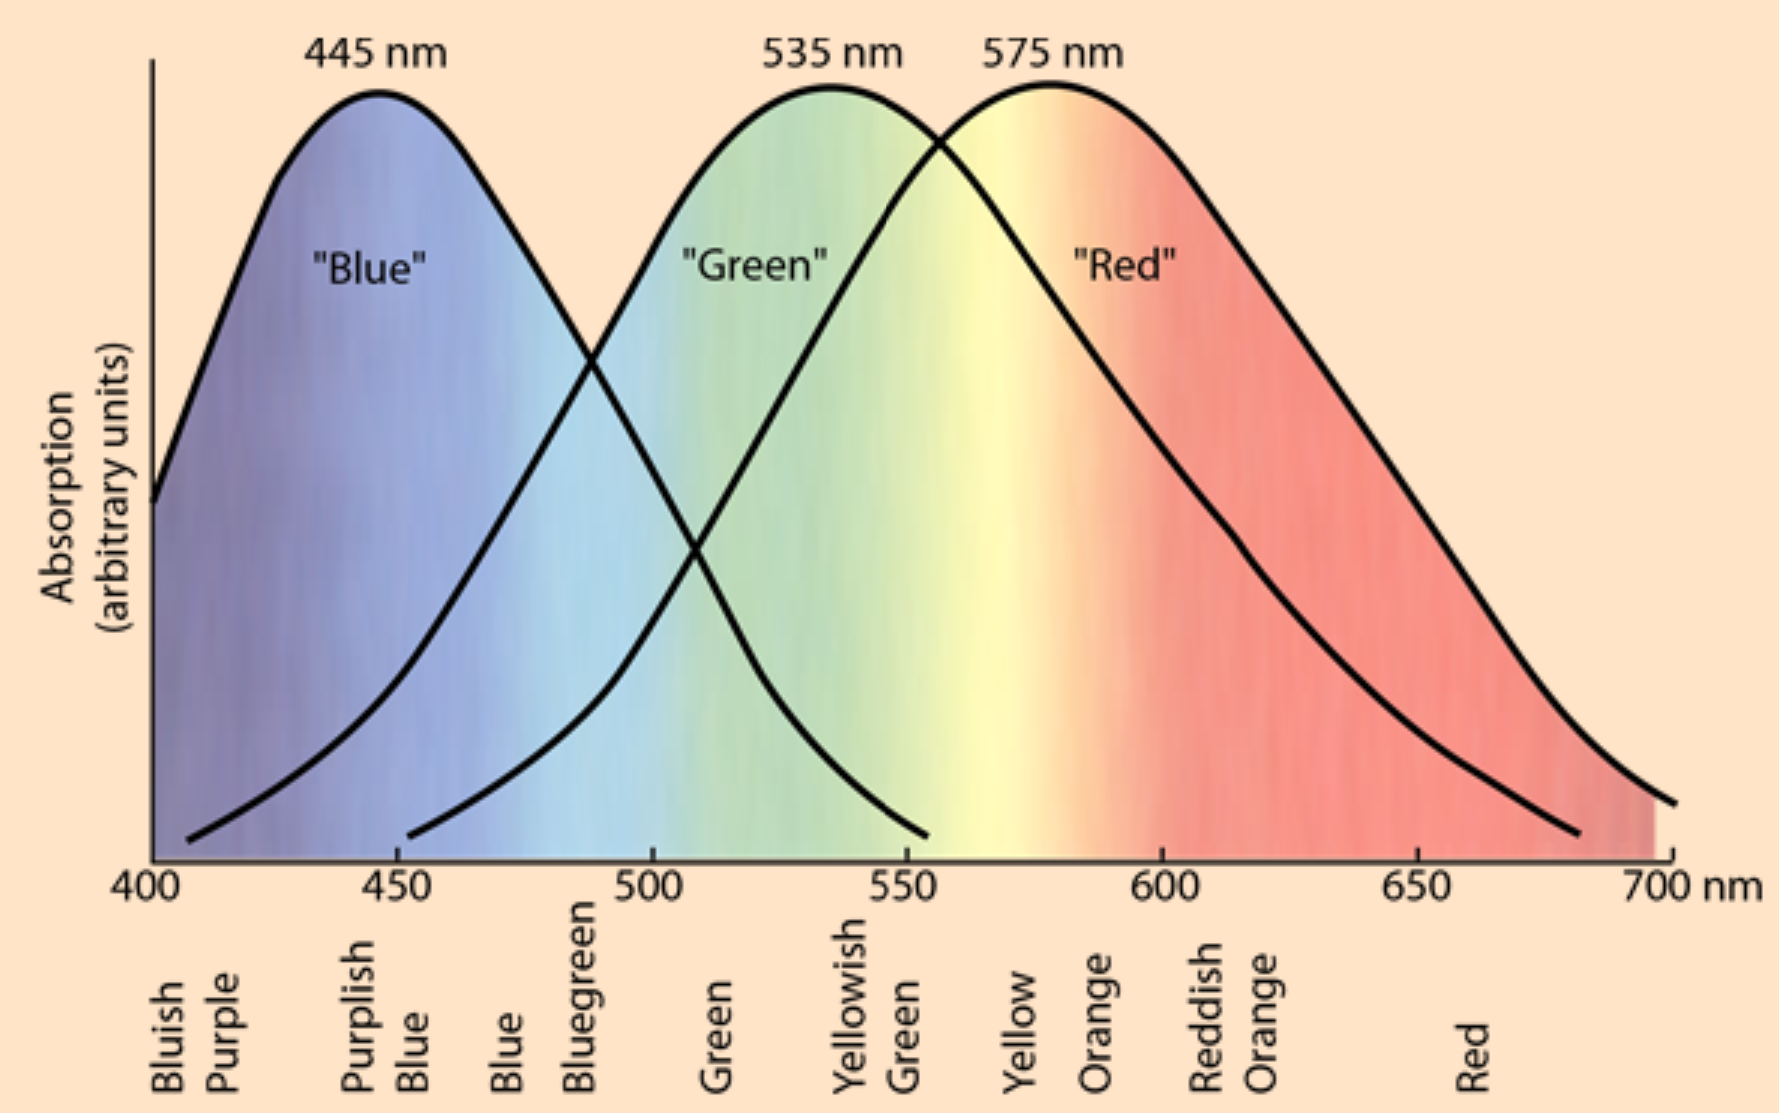
\includegraphics[width=0.75\textwidth]{figs/distribution.png}
    \caption{Typical activation distribution per cone cell type of a human eye \cite{coneinfo}}
    \label{fig:typical_activation_distribution}
\end{figure}

Our model attempts to simulate this perception and categorization of color based on wavelength. There is a lack of this type of data, so we simulate the behavior of cone cells to generate data. This data is then used to train a neural network to identify a color categorization given cell activations. An example involves selecting a wavelength (such as 560 nanometers [nm]), classifying it (yellow), and determining cone cell activations given that wavelength. The model then, given the cell activations, will ideally be able to predict and correctly recover the color classification (yellow).

\bigskip

Additionally, we introduce various types of imperfect behavior, such as dead cells, variation between individuals' unique activation distributions, and improper distribution ranges that lead to dichromacy (colorblindness) and tetrachromacy, or the possession of two or four cone cell types, respectively, rather than the typical three (trichromacy).

\section{Methods}

A variety of methods are used to both simulate and model the perception of color. At the lowest level, each individual cone cell is modeled. Together, a collection of cells is used to represent an "eye". This collection can be used to generate cell activation data. Finally, this data is used to model the perception and categorization of color. For the actual modeling of color perception, we decided to use a neural network. Our network consisted of an input layer with the dimensionality equivalent to the number of cells being modeled (i.e. if 10,000 cells are being used, the input layer has a dimensionality of 10,000), and an output layer with a dimensionality equivalent to the number of color categorization bins (i.e. if 6 colors exist, the output layer has a dimensionality of 6). The output layer will return a vector with one of the indices set to 1, corresponding to the perceived color, and all other elements set to 0.

\subsection{Virtual Cone Cell}

The smallest individual unit simulated is a virtual representation of a single cone cell. The cell is not assigned a type explicitly (i.e., L, M, or S). Instead, it is given a range of wavelengths at which it will activate.

\subsubsection{Activation Distribution}

Each cone cell type has a characteristic activation mapping from wavelength to intensity. This varies from person to person, as well as between sources (\cite{conespectra}, \cite{colorperception}, \cite{coneinfo}), but a general range of acceptable values was gathered. The activation mappings are very specific functions. That is, they can't be represented one-to-one by an easy-to-formulate equation. We noted, however, that they resemble normal distributions, and so we approximated them as such. An acceptable peak value for the respective cone cell type was used as the mean of the distribution. We were unable to find scientifically verifiable standard deviation values (as the cell response doesn't truly follow a normal distribution as mentioned earlier, so it isn't commonly classified in this way), and so we tested different values until reaching a distribution coverage that subjectively matched the measured real-world activation distributions. An example distribution can be seen below in Figure \ref{fig:simulated_distribution}. This was plotted by sampling a number of wavelengths and counting how many of each cell type were activated. To obtain the activation range of an individual cell, two values were sampled from the normal distribution corresponding to its type, with the lower value set as the minimum wavelength that activates the cell and the higher value set as the maximum wavelength that activates the cell. 

\bigskip

It is important to note that these distributions used for cone cell creation model the large scale behavior of many cone cells. Each individual cell, however, is deterministic. It has its set activation range, and will either fully activate or not activate at all, based on incoming wavelength. Varied activation levels for a cell type are only seen at a large scale.

\begin{figure}[H]
    \centering
    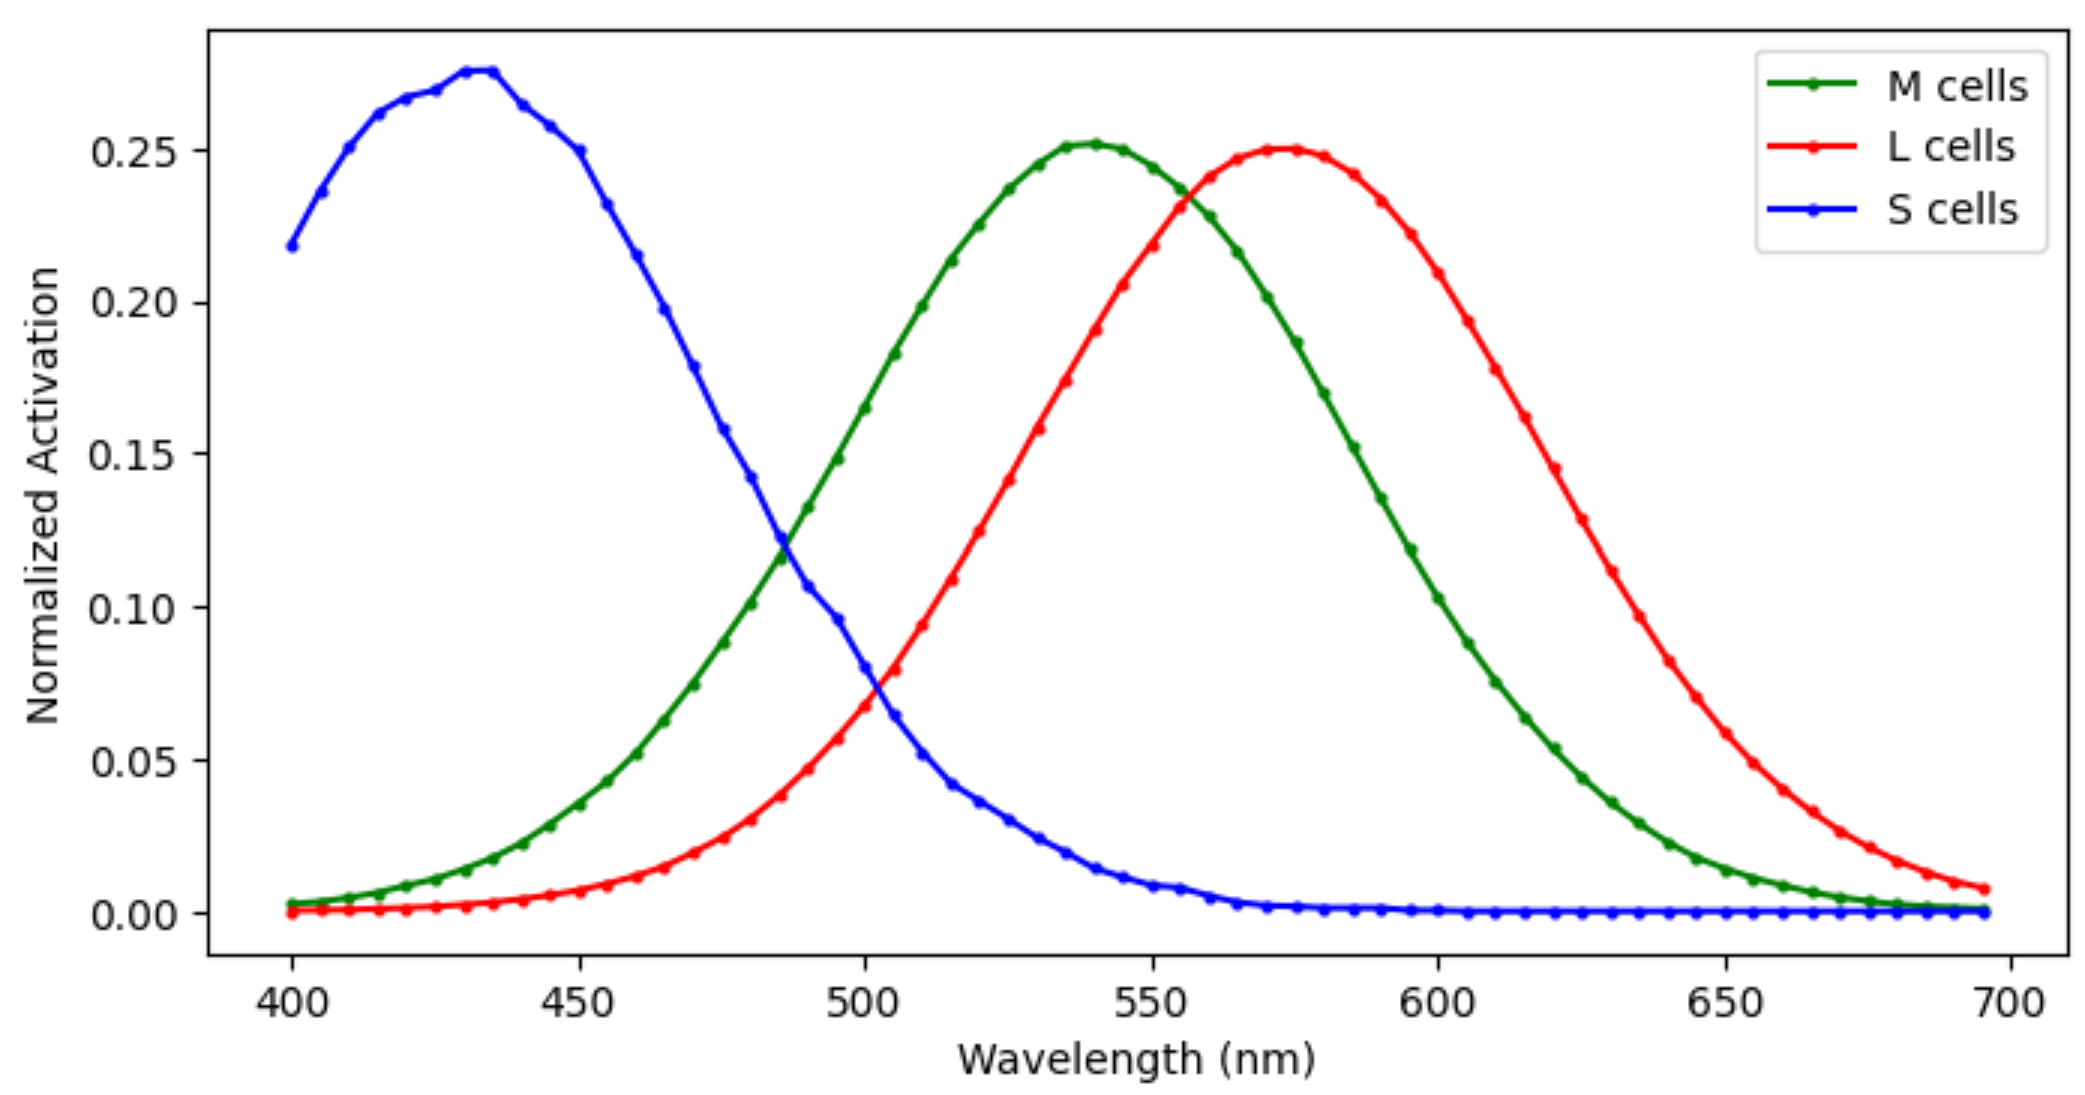
\includegraphics[width=0.75\textwidth]{figs/simulated_distribution.png}
    \caption{Normalized simulated distribution of cone cell types}
    \label{fig:simulated_distribution}
\end{figure}

\subsubsection{Cell Death}

Additionally, the status of being a "living" or "dead" cell was implemented to simulate the improper behavior of cell activations. A certain percentage of cells could be created as dead cells, which won't ever activate. This would add noise to the generated data, allowing us to see the impact of inactive cells on color perception. Living cells activate as previously described, whenever an input wavelength is within their activation range.

\subsubsection{Collection of Cells}

A large number of cells were created and interacted with for the simulation. A typical human eye has 6-7 million cone cells \cite{conebreakdown}. We decided to reduce this in our simulation as the dimensionality of the first neural network layer is directly tied to the number of cells. We did, however, ensure that the distribution of cell types was kept proportional to human eyes, with 65\% of the collection consisting of L cells, 33\% consisting of M cells, and 2\% consisting of S cells. 

\subsection{Data Generation}

We determined that the exact type of real data we required for the model was not available from a verified scientific source. This was the motivation for using a simulation to generate data. The overall process of data generation consists of two stages. 

\subsubsection{Stage 1: Cell Generation}

First, a collection of cone cells is generated. This stage is key to determining the behavior of the eye being modeled. Different eye types will be discussed below. A set number of cone cells to model is decided, we commonly used 1500. Then, based on the proportion of each cell type, the correct amount of each type is created and stored in an array. This collection is implicitly sorted by generating one cell type at a time and then concatenating all types into one list. This order gives the model insight into which cells have been activated rather than just a total number of cells activated.

\subsubsection{Stage 2: Data Collection}

The second stage involves gathering the responses of the collection of cells. This is done by first gathering a selection of random colors from our subset of colors. We specifically use red, orange, yellow, green, blue, and violet. These colors are then used to generate a corresponding wavelength based upon the wavelengths that they encompass. For example, if yellow is randomly chosen, then it will be used to generate a wavelength within its distribution, e.g. 570-590nm. The wavelength is chosen from a uniform distribution. This wavelength is compared with each cell's activation range, and a vector with the dimensionality of the number of cells is constructed. A vector index will have a value of 0 if the cell corresponding to that index \textit{did not} activate from that wavelength, or a value of 1 if the corresponding cell \textit{did} activate at that wavelength. To simulate the "all-or-nothing" activation of real cells, virtual cone cells will always fully activate or not activate at all based solely on wavelength and if the cell is living.

\subsubsection{Typical Data}

Typical data is generated as described above. Three cell types are used (L, M, S), and all cells are living. Variation is still possible with the number of eyes used for training. An eye can be thought of as a unique collection of cone cells. Since cone cells are randomly generated following a normal distribution, regenerating a collection of cells results in inherently different cells with (albeit, slightly) different activation wavelengths. To keep an eye consistent, we save it to a file to be utilized multiple times rather than regenerating it every run. To go further, as mentioned above, the peak activation for each cell type varies from person to person. Therefore, more significantly different eyes can be modeled by selecting different peak activation wavelengths. These peaks are sampled from uniform distributions over the acceptable peak range for a cell type. 

\bigskip

Models trained on a single eye are very accurate, as the probabilistic portion of the model drops out and it becomes much closer to a direct mathematical formula. Therefore, to make the problem more difficult, various eyes were used to generate the data, requiring the model to handle greater variability in the classification of color. Additionally, we investigated testing the model using data generated from both the eyes that it was trained on, as well as new eyes that the model never saw, in order to test the generalization to any (valid) abstract eye.

\subsubsection{Cell Death}

Cell death data was generated similar to typical eye data. However, the cells were given a non-zero chance of being dead on creation. These dead cells would not activate for any wavelength. For example, setting the chance of cell death to 25\% results in the creation of 25\% of all cells as dead cells. We tested and compared various rates of cell death.

\subsubsection{Dichromacy (Colorblindness)}

Various types of colorblindness are caused due to a lack of or the improper behavior of one or more cone cell types. The case we looked at isn't true dichromacy (where only two cone cell types exist). Rather, we looked at \textit{anomalous trichromacy}, in which individuals have L and M type cone cells with very similar distributions \cite{colorblindgenetics}. This leads to a reduced accuracy of color differentiation in humans, as the overlapping L and M cells respond similarly to various wavelengths (particularly red-green), leading to a lower acuity when perceiving color (as there are only two-channels present rather than three). An example this distribution can be seen below in Figure \ref{fig:dichromatic_distribution}. 

\begin{figure}[H]
    \centering
    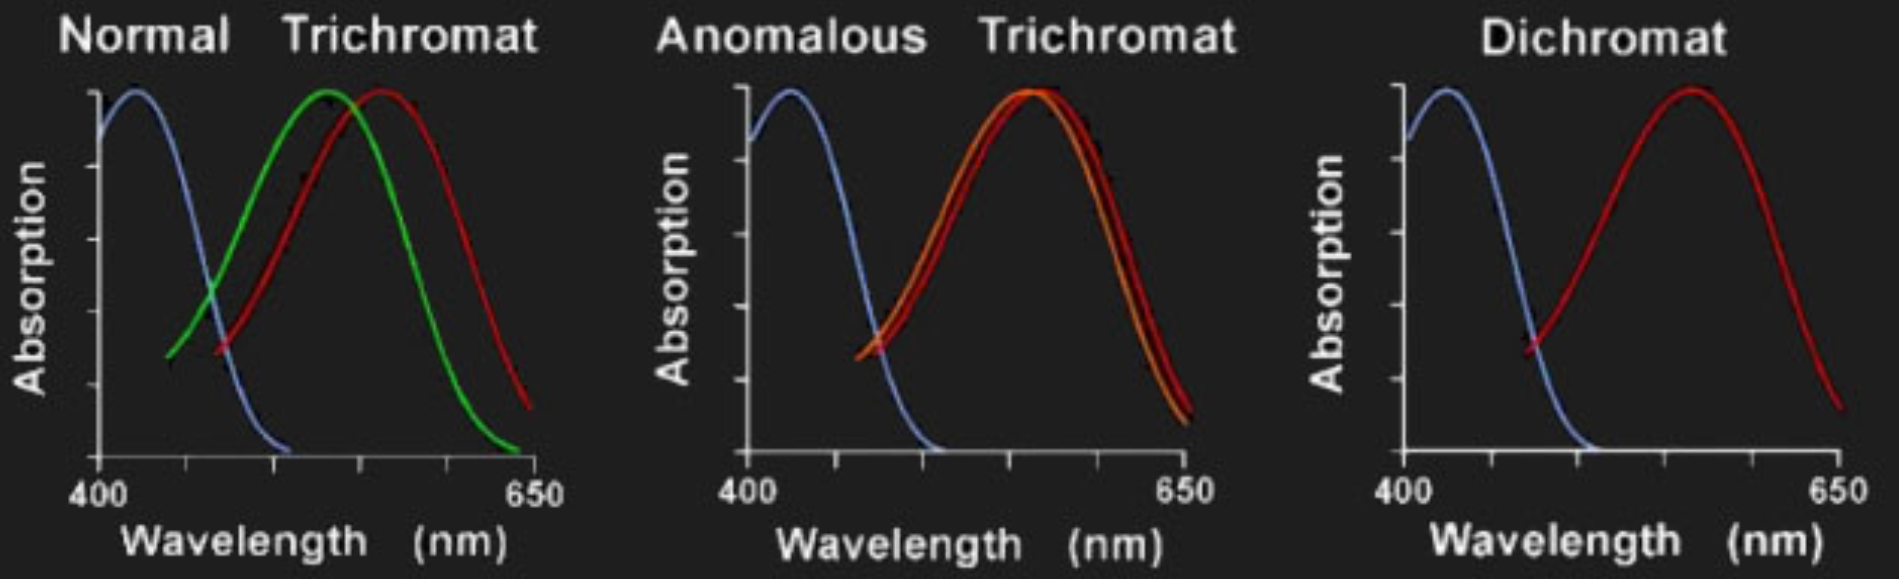
\includegraphics[width=0.75\textwidth]{figs/dichromatic_distribution.png}
    \caption{Comparison between activation distributions of typical trichromatic, anomalous trichromatic, and true dichromatic eyes \cite{anamoloustri}}
    \label{fig:dichromatic_distribution}
\end{figure}

We simulated these types of eyes by averaging the peak activation wavelengths for L and M cone cells and creating an eye consisting of two types of cells, with S cells making up 2\% of the retina and L/M cells making up the remaining 98\%. An example of this can be seen below in Figure \ref{fig:our_dichromatic}.

\begin{figure}[H]
    \centering
    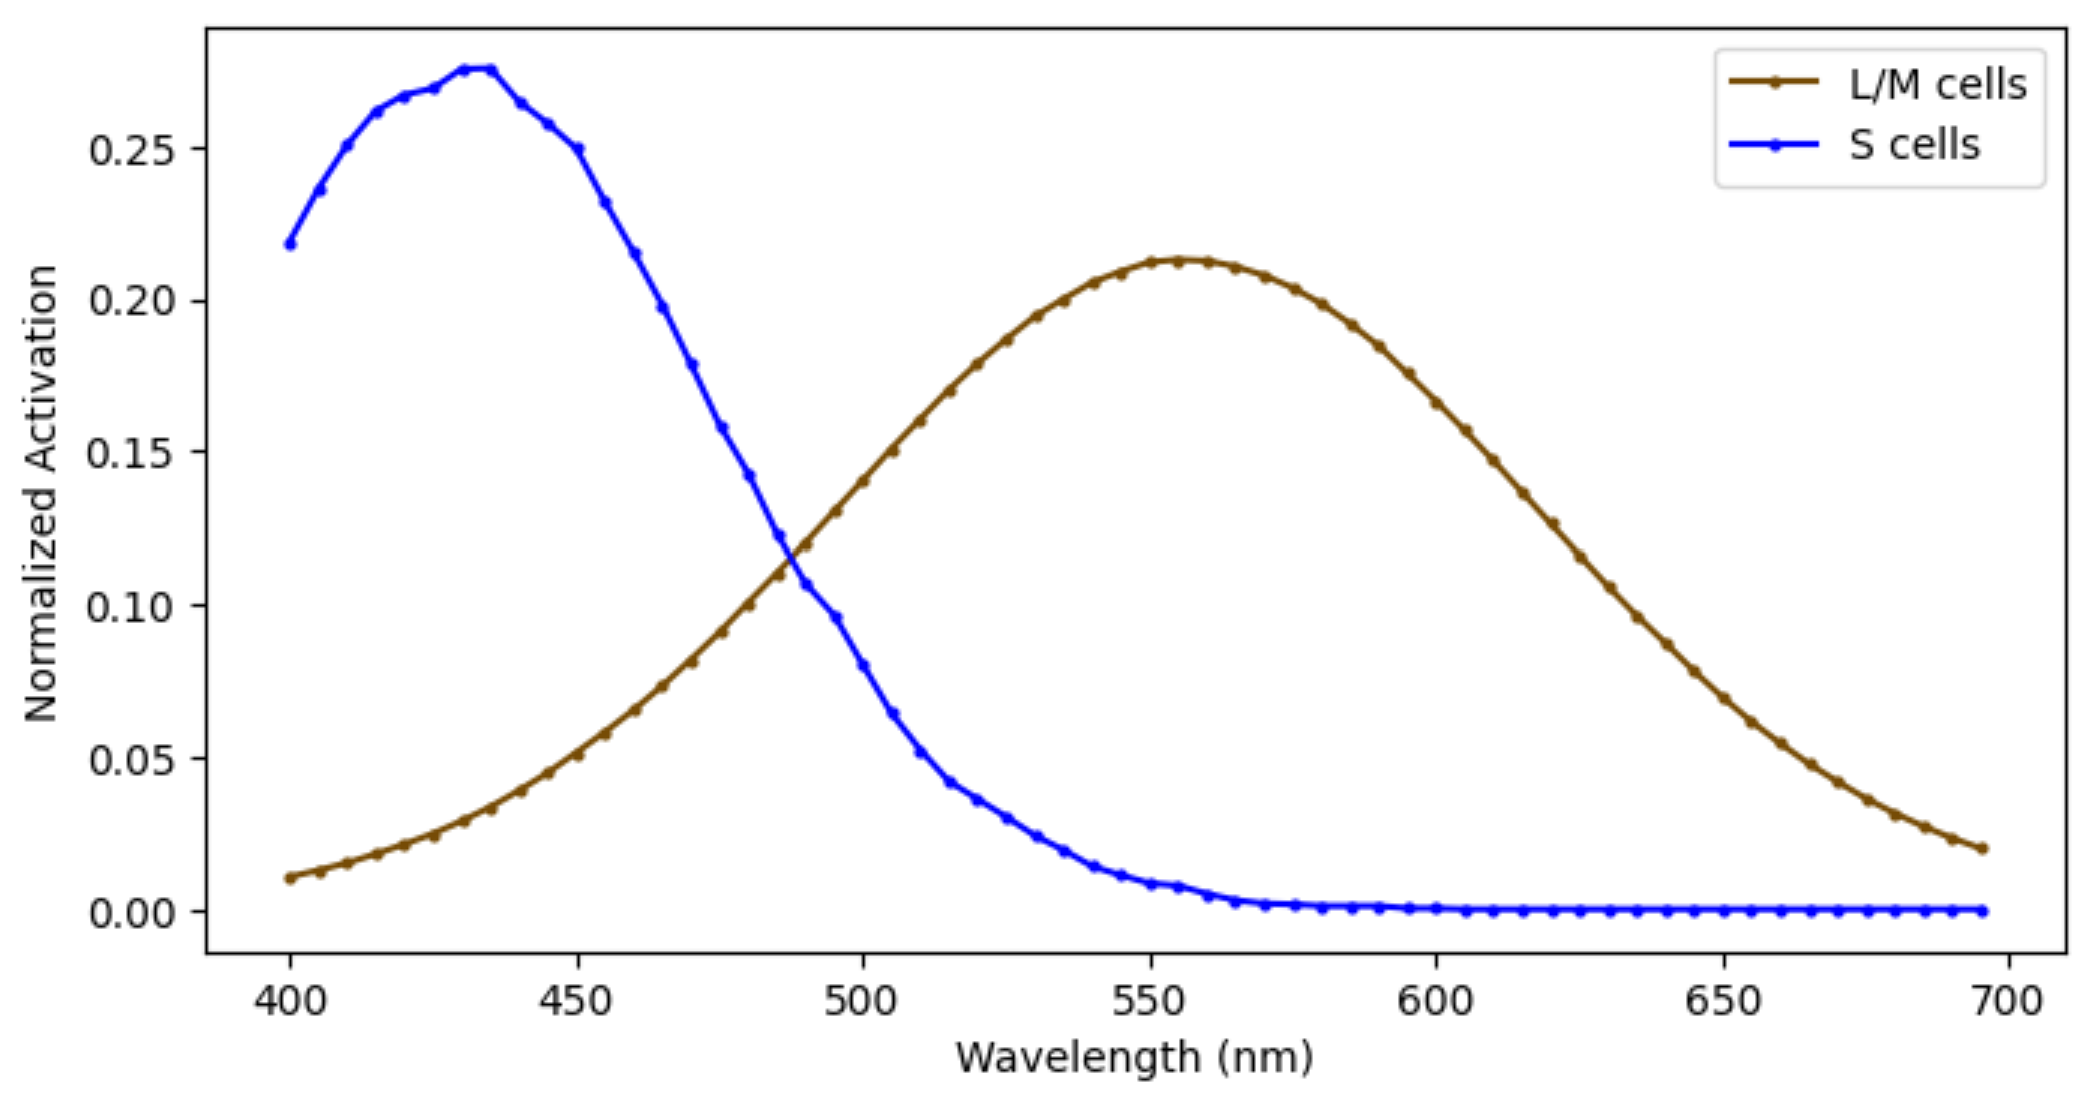
\includegraphics[width=0.75\textwidth]{figs/our_dichromatic.png}
    \caption{Example normalized distribution representative of colorblindness used in the model}
    \label{fig:our_dichromatic}
\end{figure}

\subsubsection{Tetrachromacy}

Tetrachromacy refers to the condition of having four distinct cone cell types. Humans with this condition inherit a regular M cone cell type from the mother and a mutated M cone cell type from their father \cite{tetragenetics}. This mutated cell type has a peak frequency in between the typical M and L type peaks, acting as a fourth cell type. Due to the position of this fourth cone cell's peak activation on the wavelength domain, it doesn't offer a massive enhancement of color perception. Rather, it slightly enhances the ability to distinguish between already visible shades, particularly for longer wavelengths (warmer colors, as that is where the fourth cell's peak is located). An example tetrachromatic distribution can be seen below in Figure \ref{fig:tetrachromatic_distribution}. 

\begin{figure}[H]
    \centering
    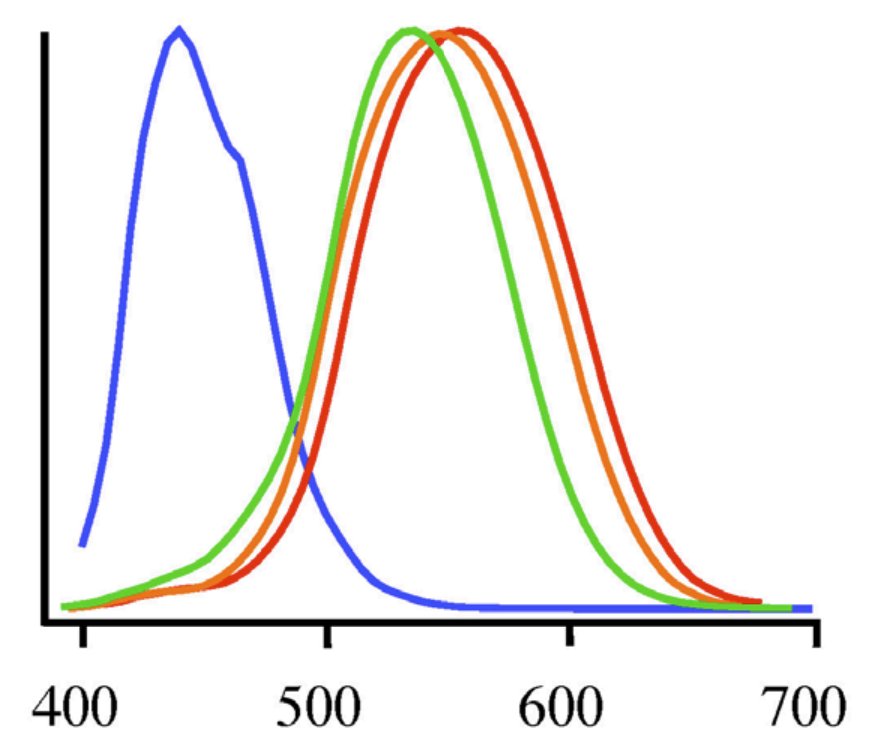
\includegraphics[width=0.5\textwidth]{figs/tetrachromatic_distribution.png}
    \caption{Tetrachromatic distribution \cite{tetragraph}}
    \label{fig:tetrachromatic_distribution}
\end{figure}

We model this cell type using a fourth cone cell distribution with peak activation wavelengths ranging between 550nm and 560nm. We were unable to find a scientifically verifiable accounting for the number of these cells, but due to the genetic reasoning for their existence, we decided to take half of the M cone cells (that would be from the father) and turn them into the fourth variant, M'. Therefore, the new distribution consists of 65\% L cells, 16.5\% M cells, 16.5\% M' cells, and 2\% S cells. An example distribution representative of the tetrachromatic model can be seen below in Figure \ref{fig:our_tetrachromatic}. 

\begin{figure}[H]
    \centering
    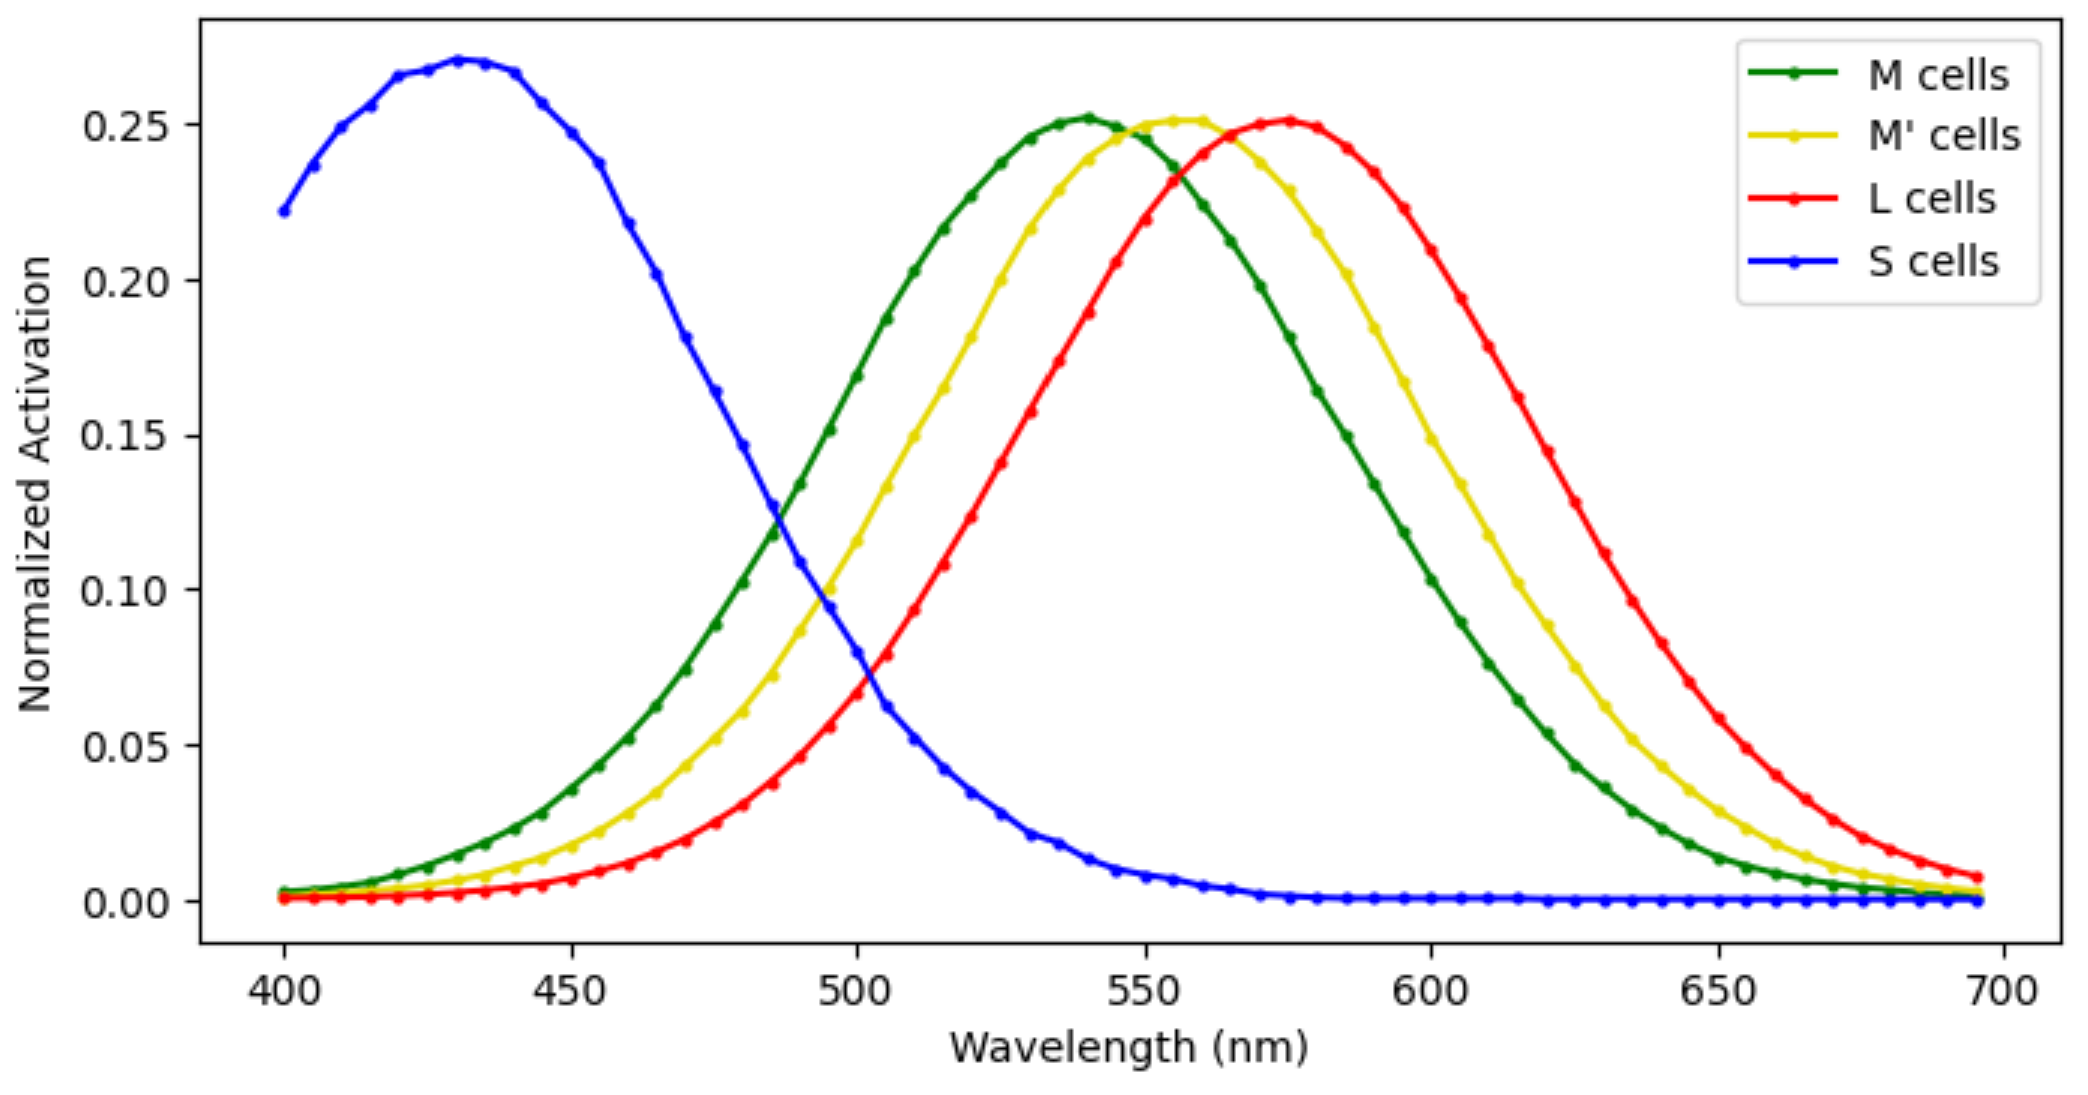
\includegraphics[width=0.75\textwidth]{figs/our_tetrachromatic.png}
    \caption{Example distribution representative of tetrachromacy}
    \label{fig:our_tetrachromatic}
\end{figure}

\subsection{Model}

We used a neural network to model the categorization of color based on the activation of the cone cells. Specifically, we used the \lstinline{keras} Python library. We were primarily interested in how the design of the network impacted the validity of its predictions. We also examined how the model reacted to new eyes of the same and different types.

\subsubsection{Configuration}

The network consists of eight \lstinline{Dense} layers using 256 units and the Sigmoid Linear Unit (\lstinline{"silu"}) activation function. Between each \lstinline{Dense} layer is a \lstinline{Dropout} layer with a rate of 0.2. These \lstinline{Dropout} layers help to prevent overfitting in the model. The final layer uses the \lstinline{"softmax"} activation function in order to produce a probabilistic distribution. This distribution can then be used to determine which color was predicted.

\bigskip

The \lstinline{AdamW} optimizer was used with a learning rate of 5e-4 and a weight decay of 0.004. The model was trained for a total of 20 epochs with a validation split of 0.1. The model was trained using data generated from "typical" eyes.

\bigskip

We went through multiple iterations while attempting to balance the number of eyes and the number of samples we took from each eye. Originally, we only used 10 different eyes: 8 for training and 2 for testing. For each eye, we generated samples from 1000 colors. This, however, did not provide good results. The training set has, on average, the same color from the same eye repeated 150 times. Since there are a total of 8000 samples in the training dataset, approximately 1.9\% of all samples were the same color from the same eye. This means that the effective size of the set with only unique data points is approximately 50. This was reflected in the performance of the model, with an accuracy of 50-60\% when using the test set. To fix this, the number of eyes was increased to 200, with 160 for training and 40 for testing. Additionally, the number of samples generated from each eye was limited to 15. This reduces the repetition of data significantly. Instead of the training set having the same color from the same eye 150 times, it is now just an average of 3 times.

\section{Results}

The process of formulating this model was an ongoing, iterative experience. We simultaneously wanted a model that was fairly accurate and performed well, but also a model that wasn't perfect, as that meant we weren't truly modeling any probabilistic behavior. At the start, we utilized one "eye" for training, validation, and testing. This proved to be too accurate, as the mapping for one single eye was very close to a direct mathematical formulation. This behavior is understandable in hindsight, as we are modeling the process the brain utilizes for color perception, and typical eyes in standard conditions perceive color very well. Therefore, we introduced multiple eyes, as well as using different eyes for the training and for the testing. This brought the probabilistic behavior back, where now each "cell" has a probability of activating (referring to the same positional cell across multiple eyes, i.e. the Nth S cell) instead of a single cell with a set activation range. Additionally, we introduced various forms of atypical behavior, such as the dead cells modeling noise, and using two or four cone cell types rather than three.

\subsection{Diagnostics}

Figure \ref{fig:loss_trajectory} shows the loss trajectory of the model. As can be seen, the training loss continuously decreases, while the validation loss plateaus and even increases a little. This signals overfitting in the model. This overfitting was originally much worse. It was improved by adding \lstinline{Dropout} layers to the neural network. Further attempts to prevent overfitting by removing layers or training for fewer epochs only caused a decrease in model accuracy.

\begin{figure}[H]
    \centering
    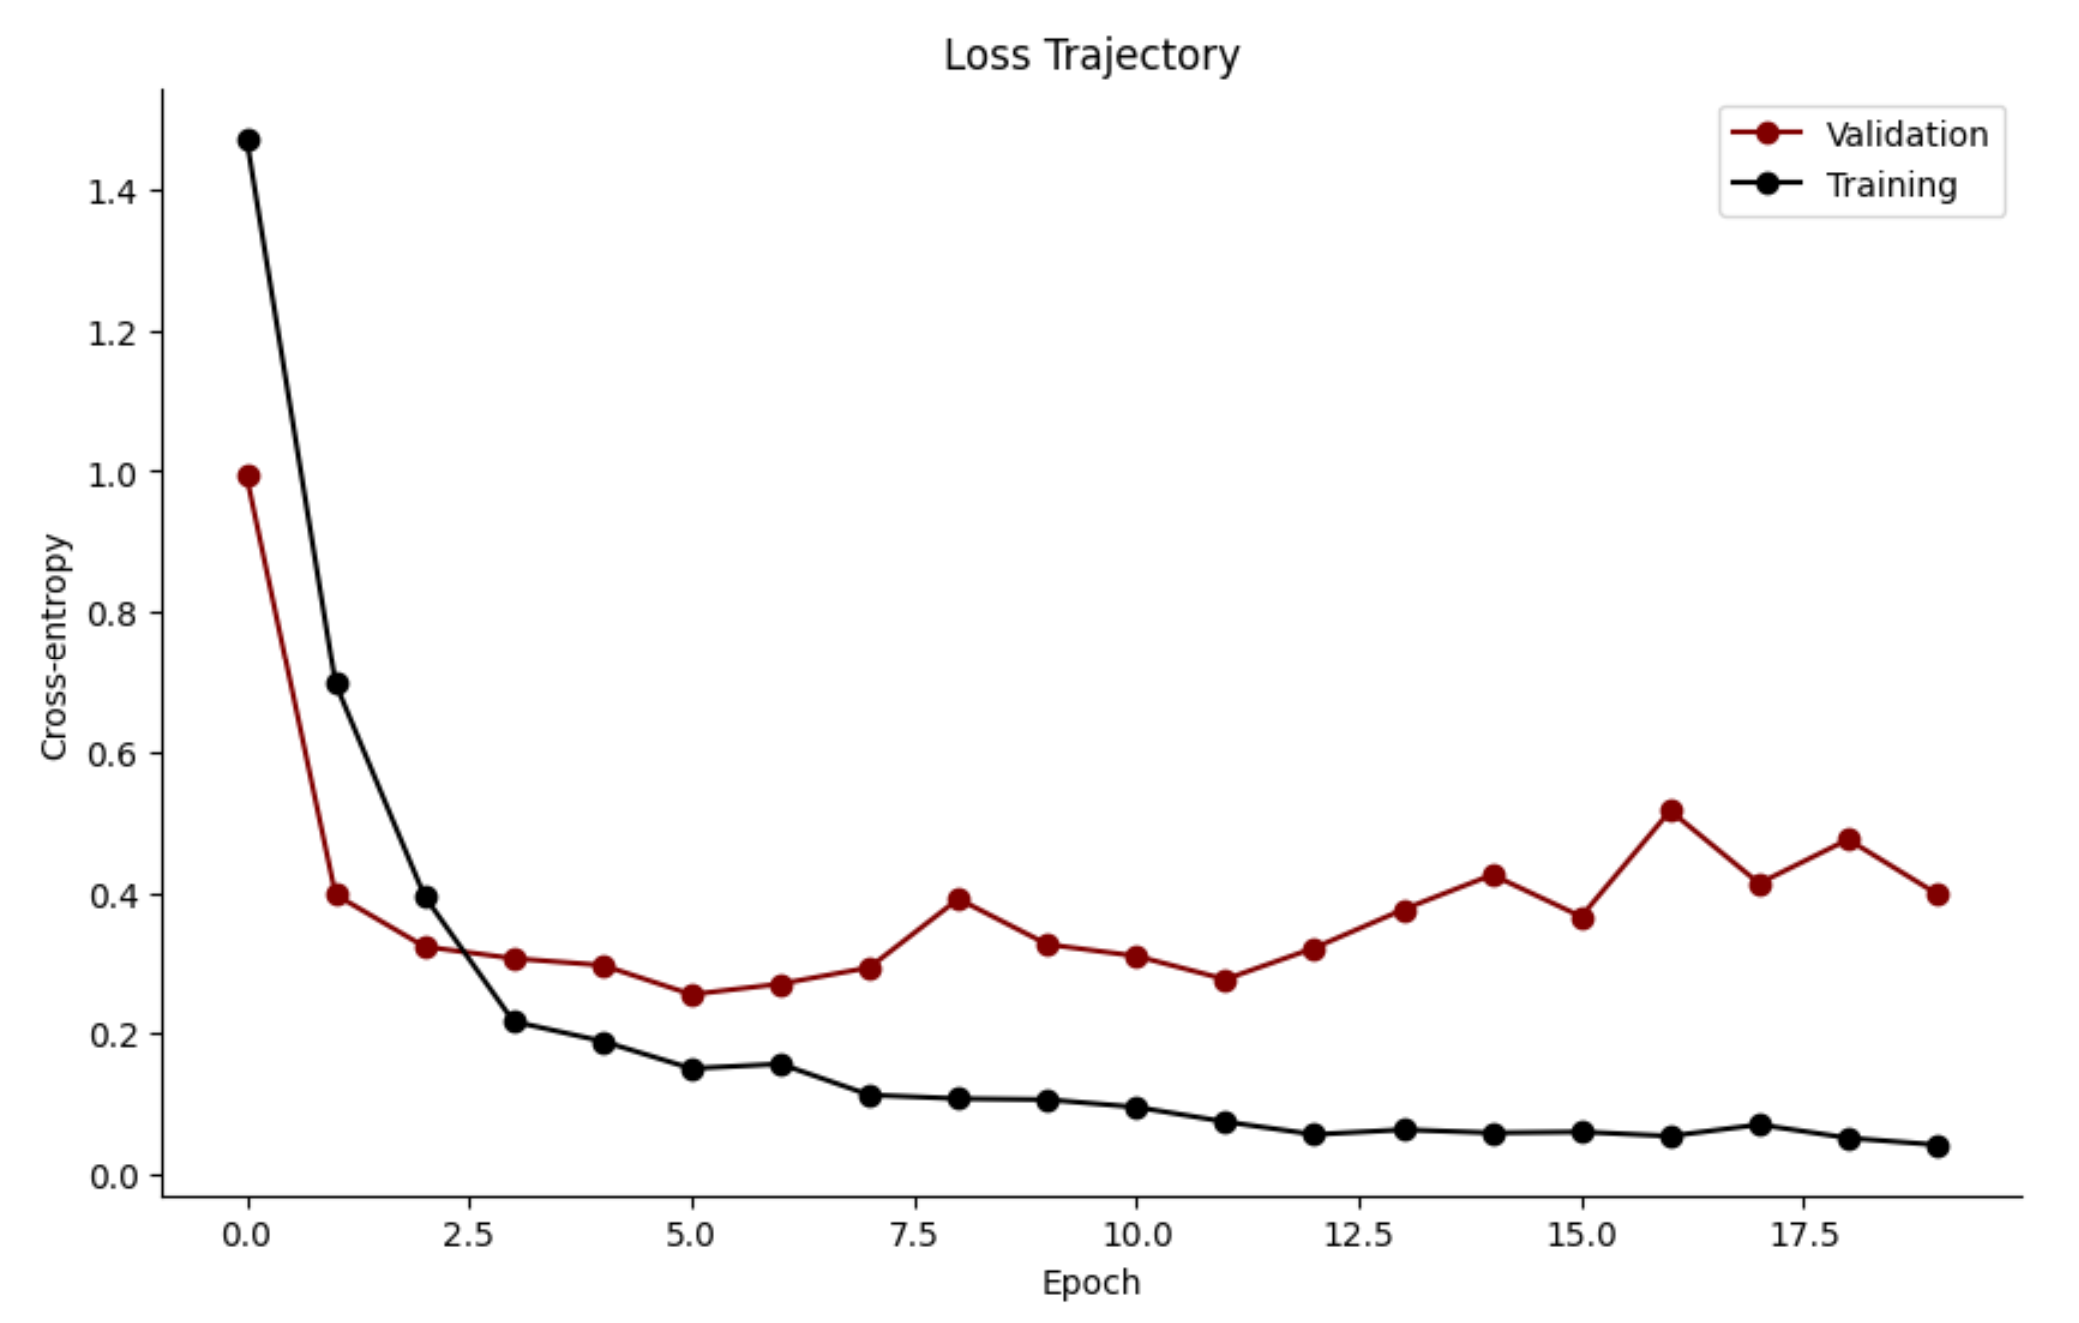
\includegraphics[width=0.75\textwidth]{figs/loss_trajectory.png}
    \caption{Loss trajectory of the model}
    \label{fig:loss_trajectory}
\end{figure}

\subsection{Interpretation}

Overall, the model performs reasonably well for the typical case. It is capable of achieving \~90\% accuracy when tested on cone cells from eyes it has never seen during training. This decreases significantly when tested on atypical eyes, which is to be expected. Based on this, we were able to accurately model the process of taking the activation levels of cone cells and mapping that to the causing color. We were also able to show the impact that different atypical eyes have on color perception.

\bigskip

Based on our modeling, one implication is that typical human eyes are similar enough that it is possible to predict any arbitrary eye's color perception based on the activation levels of the cone cells. This is, however, limited to situations in which the order of the cone cells is known, which would be rare. The model also emphasizes how much of an impact atypical eyes can have on performance, as is experienced by many people.

\subsection{Validation \& Sensitivity}

\subsubsection{Single Typical Eye and Multiple Typical Eyes}

We originally trained the model using one eye, however, the results were not interesting. Because all of the training data came from the same source, the model was able to memorize that data and repeat it during testing. The next step was training using multiple eyes. However, before we moved to separating the eyes between training and testing sets, we shuffled all eyes into both sets. This also proved to be uninteresting with pretty similar results. It was not until we decided to use entirely separate eyes for training and testing that we saw good results.

\subsubsection{Multiple Typical Eyes Validated with Different Typical Eyes}

Figure \ref{fig:typical_confusion_matrix} shows the confusion matrix for the model when tested on typical eyes it had never seen before. As can be seen, the model performed well. The incorrect predictions are all colors that are directly adjacent to their true values.

\begin{figure}[H]
    \centering
    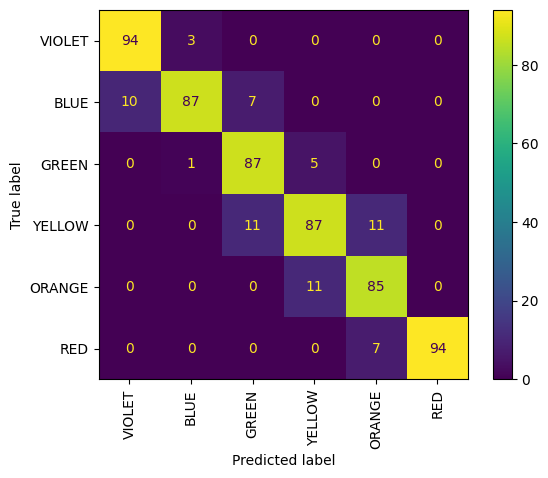
\includegraphics[width=0.75\textwidth]{figs/typical_confusion_matrix.png}
    \caption{Confusion Matrix for Testing on Typical Eyes}
    \label{fig:typical_confusion_matrix}
\end{figure}

\subsubsection{Comparison of Eyes with Varying Levels of Cell Death}

Figure \ref{fig:dead_cell_confusion_matrix} shows the confusion matrix for the model when tested on eyes with a probability of cone cells being dead. These eyes do not have a certain percentage of cone cells that are dead, but rather a probability that is evaluated for each cone cell. As can be seen, the model initially performs well. The diagonal is still relatively strong up until a probability of 0.3. When the probability is 0.4 and 0.5, the diagonal is still there, but it is much less obvious. But, from 0.6 and on, the diagonal does not exist at all.

\begin{figure}
    \centering
    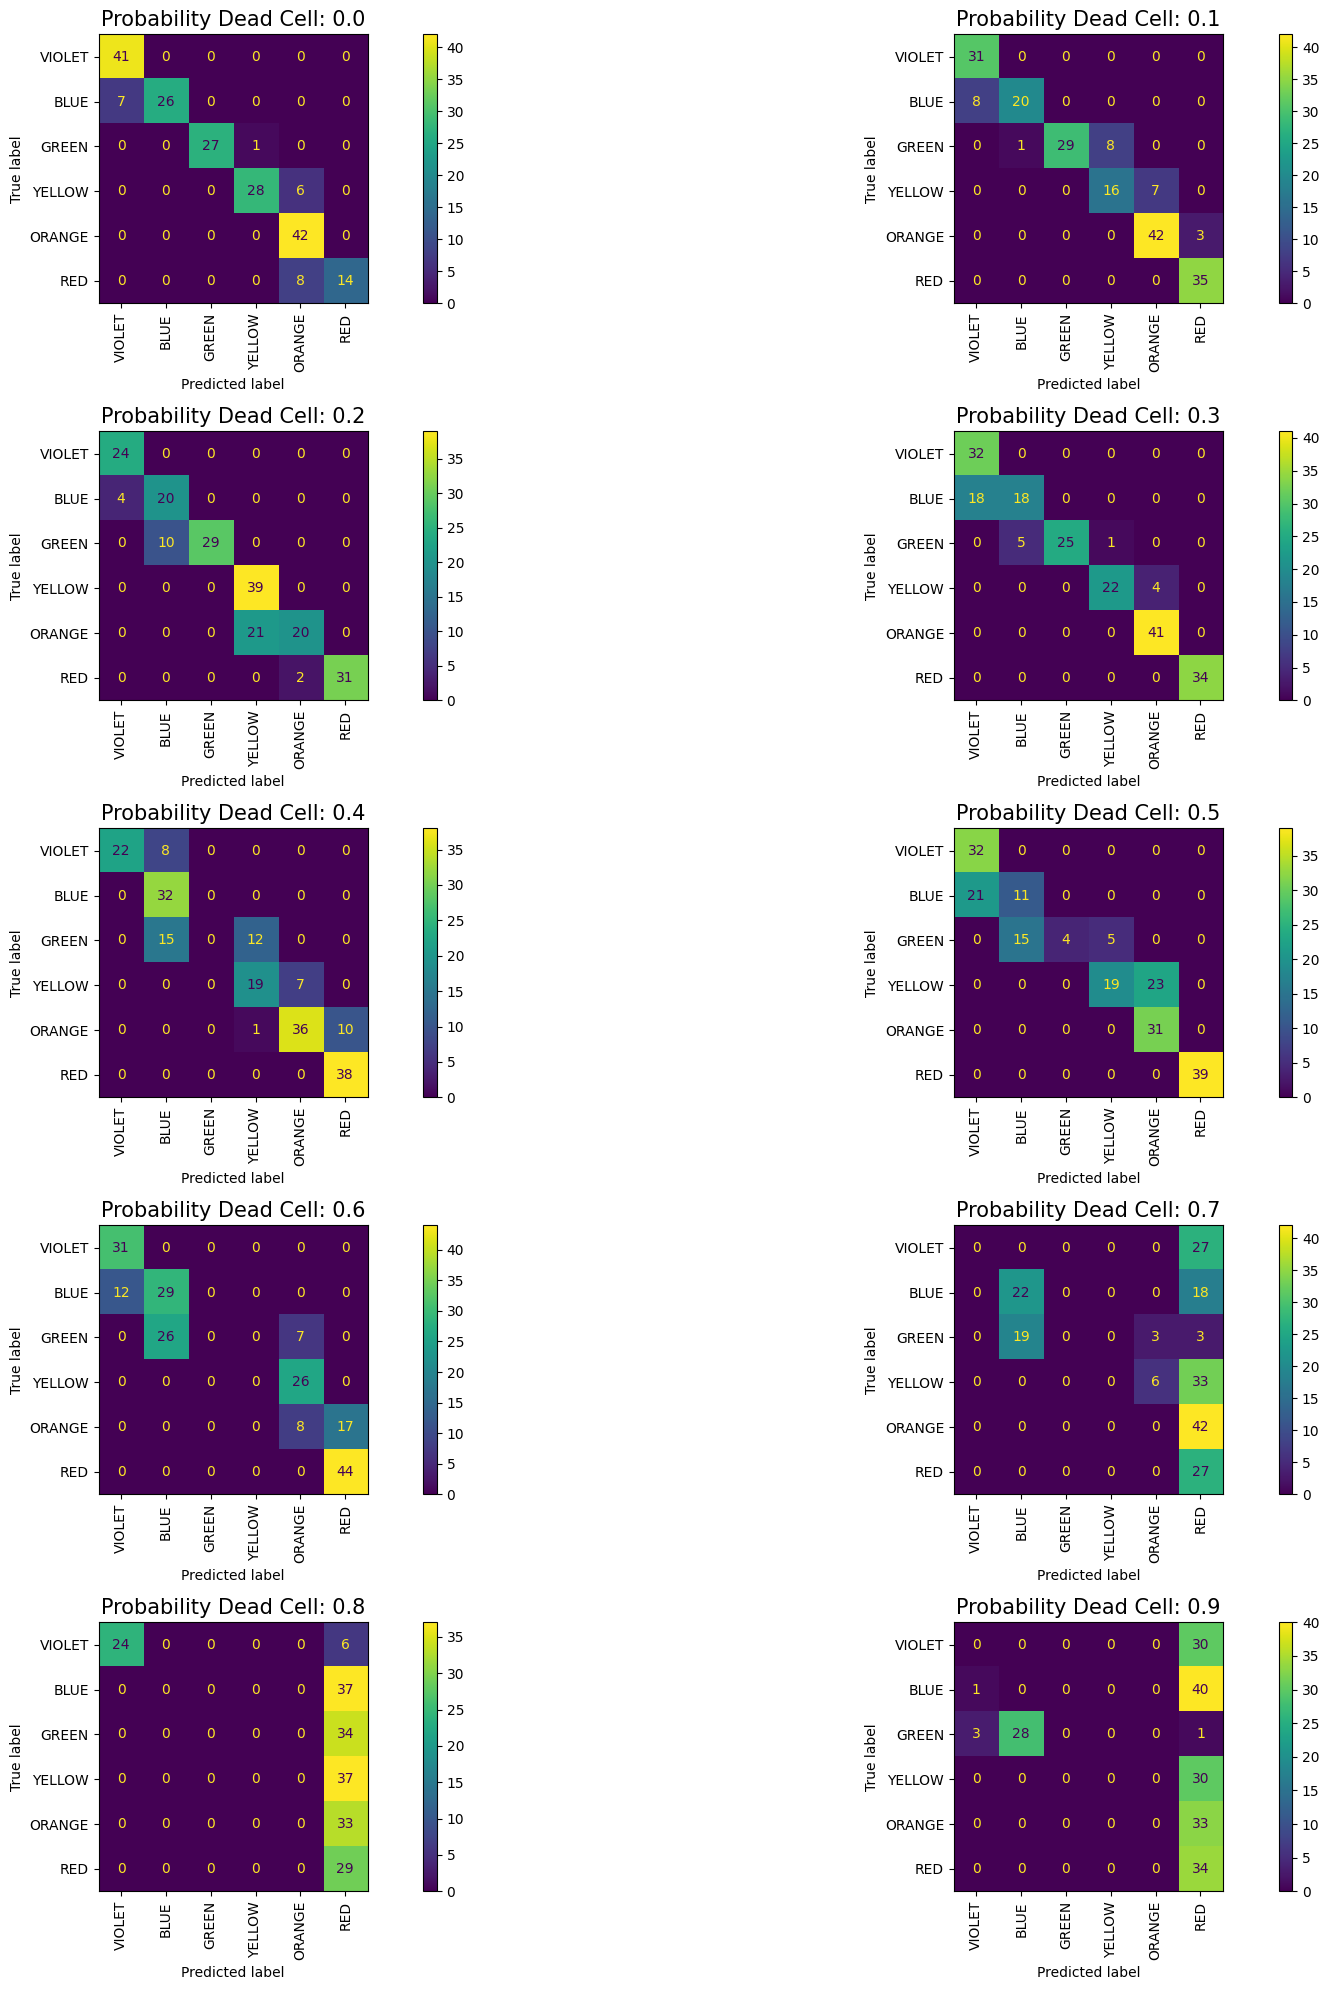
\includegraphics[width=\textwidth]{figs/dead_cell_confusion_matrix.png}
    \caption{Confusion Matrix for Testing on Eyes with Progressively more Dead Cells}
    \label{fig:dead_cell_confusion_matrix}
\end{figure}

Figure \ref{fig:dead_cell_accuracy} shows the accuracy of the model as the probability of cells being dead increases. The general trend is that higher the probability, the worse the accuracy. By the time the probability is at 0.8, the accuracy is so low that random chance would have similar results. For lower probabilities, i.e. 0.3-0.4 and below, the model still performs well.

\bigskip

The graph itself is highly noisy. This is due to there not being a uniform application of dead cells across cell types. For example, two eyes can have a 0.2 probability of cells being dead, and one eye has 25\% of L cells dead while the other eye only has 28\% of L cells dead. As a result, some eyes may be more affected because they lose a large number of important cells. 

\begin{figure}[H]
    \centering
    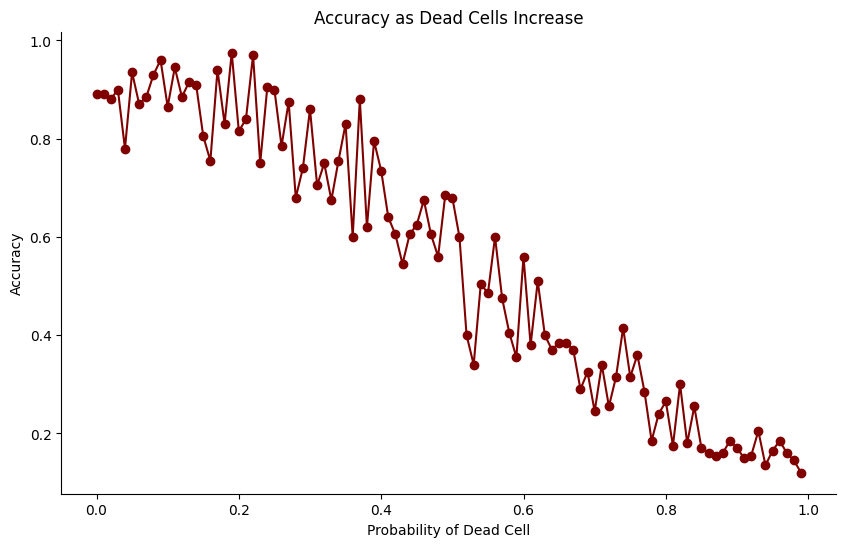
\includegraphics[width=\textwidth]{figs/dead_cell_accuracy.png}
    \caption{Accuracy of Model as Probability of Cells Being Dead Increases}
    \label{fig:dead_cell_accuracy}
\end{figure}

\subsubsection{Dichromatic Eyes (2 Cell Types - Red-Green Colorblind)}

Figure \ref{fig:colorblind_confusion_matrix} shows four examples of confusion matrices for colorblind eyes. The results are both expected and surprising. Colors that should be on the warmer side (i.e. red, orange, and yellow) have predictions that are shifted towards the cooler side. Since the type of colorblindness we modeled was red-green colorblind, it makes sense that the model would have difficulty distinguishing reds, oranges, and yellows from greens. However, it is surprising that there are not that many cases of green colors being predicted to be reds, oranges, or yellows.

\begin{figure}[H]
    \centering
    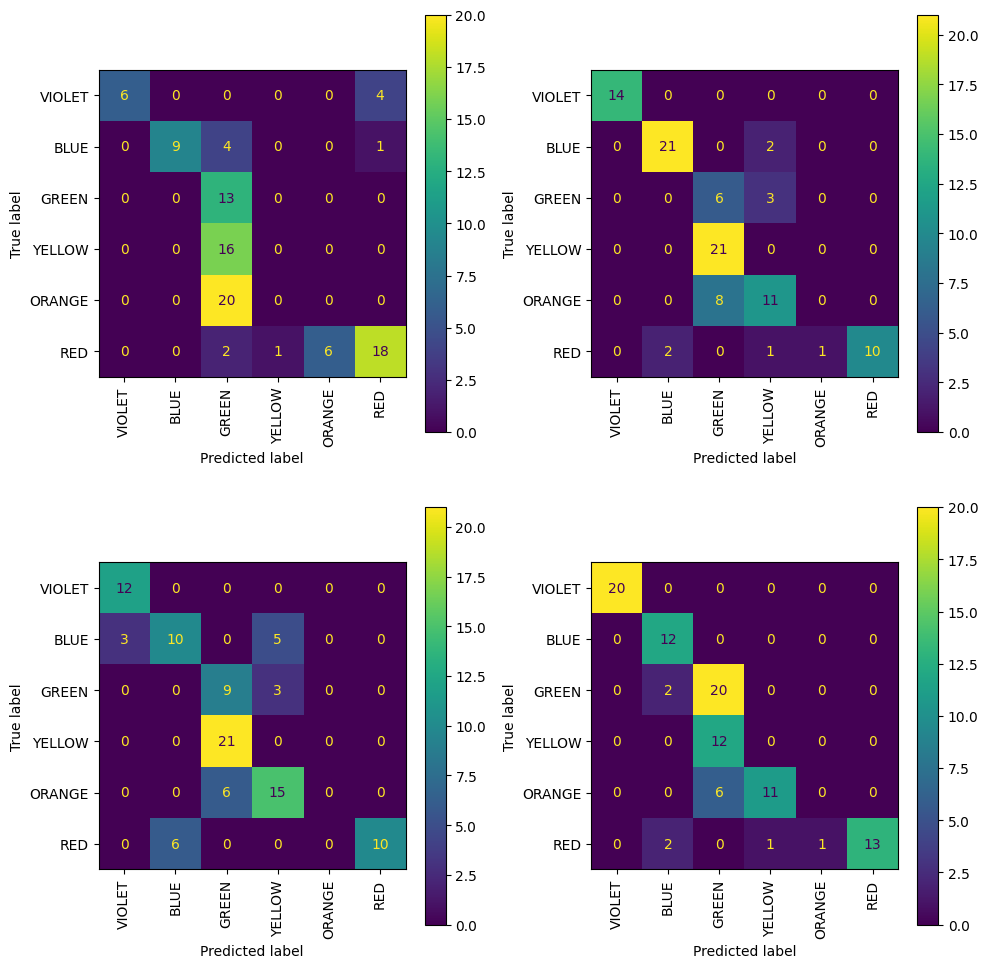
\includegraphics[width=\textwidth]{figs/colorblind_confusion_matrix.png}
    \caption{Confusion Matrix for Testing on Typical Eyes}
    \label{fig:colorblind_confusion_matrix}
\end{figure}

\subsubsection{Tetrachromatic Eyes (4 Cell Types - Additional Color Perception)}

Figure \ref{fig:tetrachromatic_confusion_matrix} shows four examples of confusion matrices for tetrachromatic eyes. The results here closely mimic the results for typical eyes. One difference, however is that yellow is not incorrectly predicted to be orange, as was the case for typical eyes. There are, however, a higher percentage of oranges predicted to be yellow. This makes sense for tetrachromatic eyes, as the fourth type of cone cell peaks around the wavelengths for yellow.

\begin{figure}[H]
    \centering
    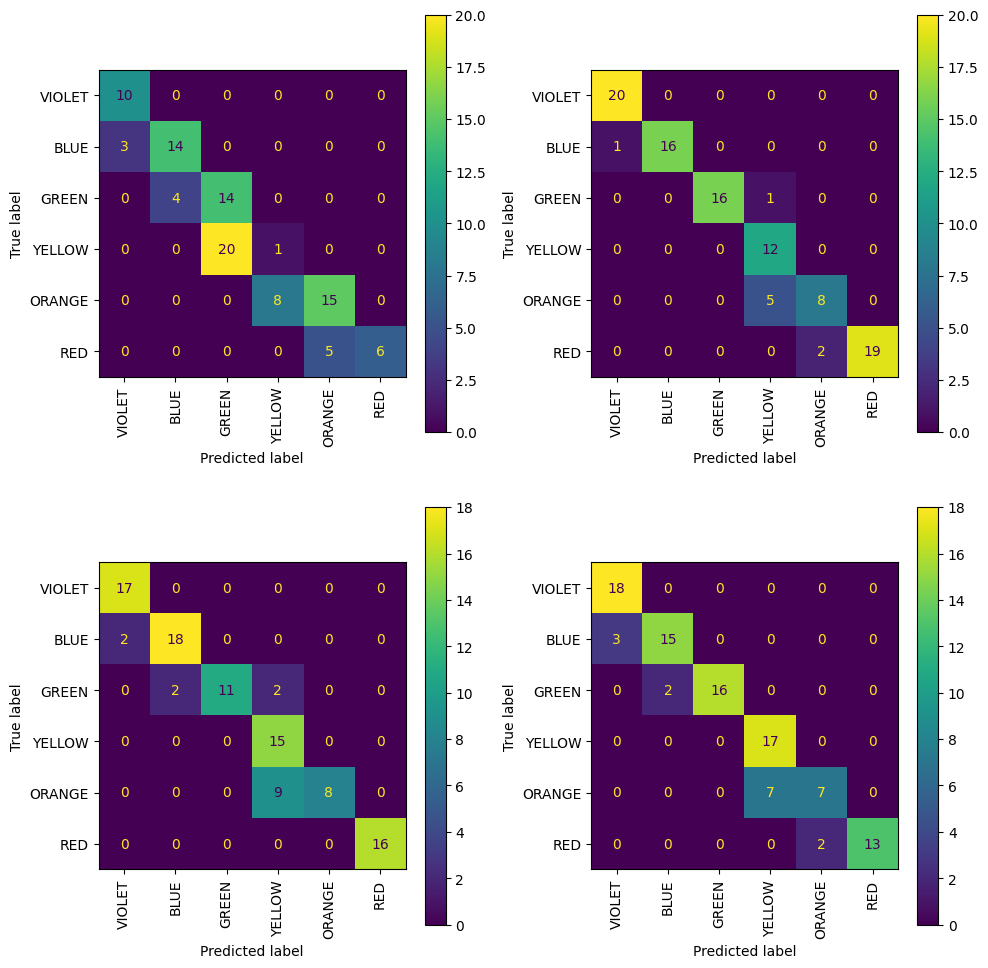
\includegraphics[width=\textwidth]{figs/tetrachromatic_confusion_matrix.png}
    \caption{Confusion Matrix for Testing on Typical Eyes}
    \label{fig:tetrachromatic_confusion_matrix}
\end{figure}

\subsection{Visualization}

We devised a method of visualizing the perceptions of the model. We can take a collection of wavelengths, classify them as colors, and arrange them into an image. This is the ground truth. Then, we can obtain the model's perceptions of each wavelength and similarly arrange it as an image. This can be used to visually and intuitively observe the model's performance. This can be done with random data to pick up trends, or can be done with an image that resembles an object. We decided to showcase both, using a simple image of a flower. This visualization was done for each type of situation we trained on. The first figure will be the flower and the second figure will be noise, with the original being the leftmost image and the perceived version(s) on the right.

\bigskip

Note that no actual positional data or image exists here. Rather, a collection of independent predictions were stitched together in a way to improve the intuitive understanding of a human observer. An additional note is that these images consist of one single prediction per pixel. A more accurate interpretation could likely be found by repeating the visualization multiple times trained on different unique eyes, and averaging the results together. Different image types consisting of alternative color pallets (i.e. more warm colors vs. the high level of cool colors in the flower image) could be tested to see if trends remain.

\subsubsection{Multiple Typical Eyes}

Typical eyes were able to perfectly recreate this small image. If recreated numerous times, it's likely it will predict incorrectly occasionally, but the general perception of the image is accurate. 

\begin{figure}[H]
    \centering
    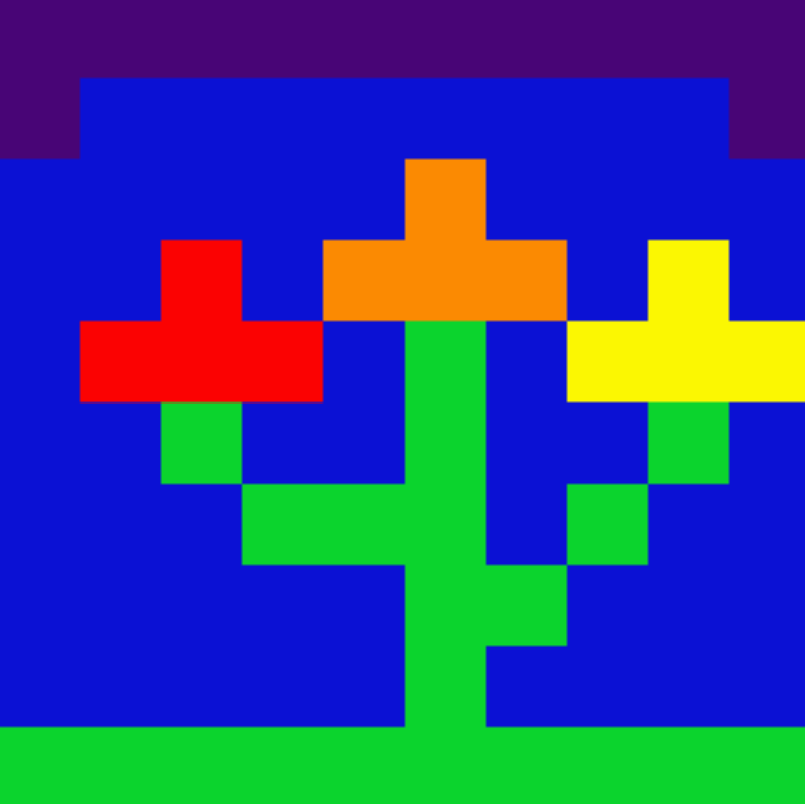
\includegraphics[width=0.2\textwidth]{figs/original_flower.png}
    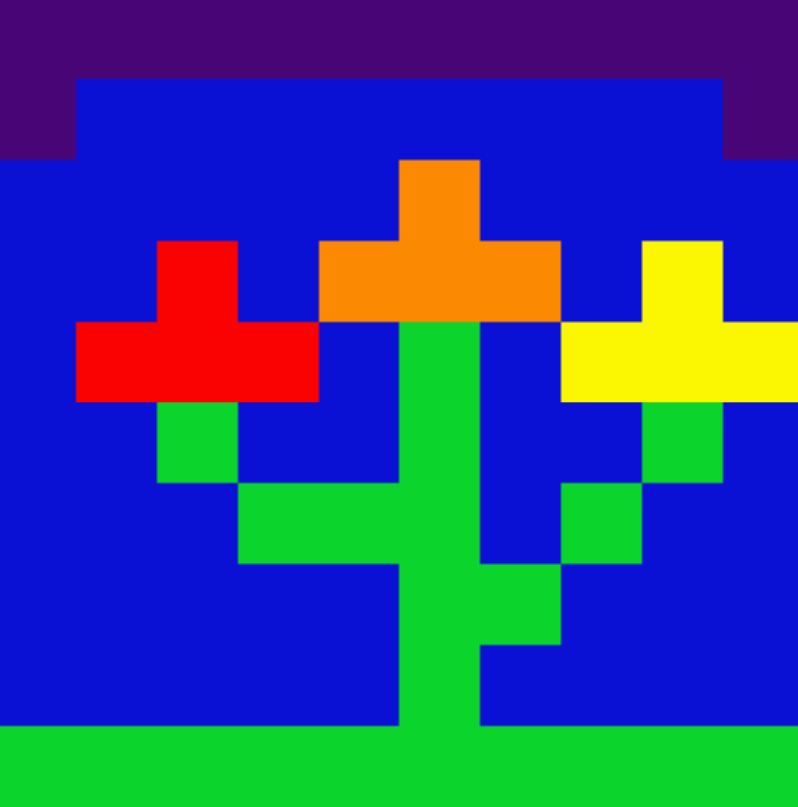
\includegraphics[width=0.2\textwidth]{figs/flower_normal.png}
    \caption{Left: Original flower. Right: Flower perceived by multiple typical eyes}
\end{figure}

\begin{figure}[H]
    \centering
    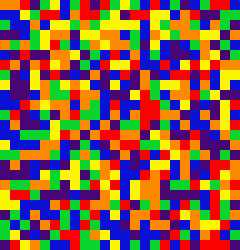
\includegraphics[width=0.2\textwidth]{figs/typical_actual_results.png}
    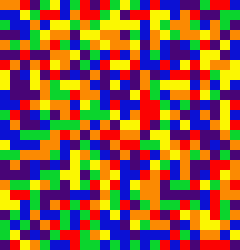
\includegraphics[width=0.2\textwidth]{figs/typical_predicted_results.png}
    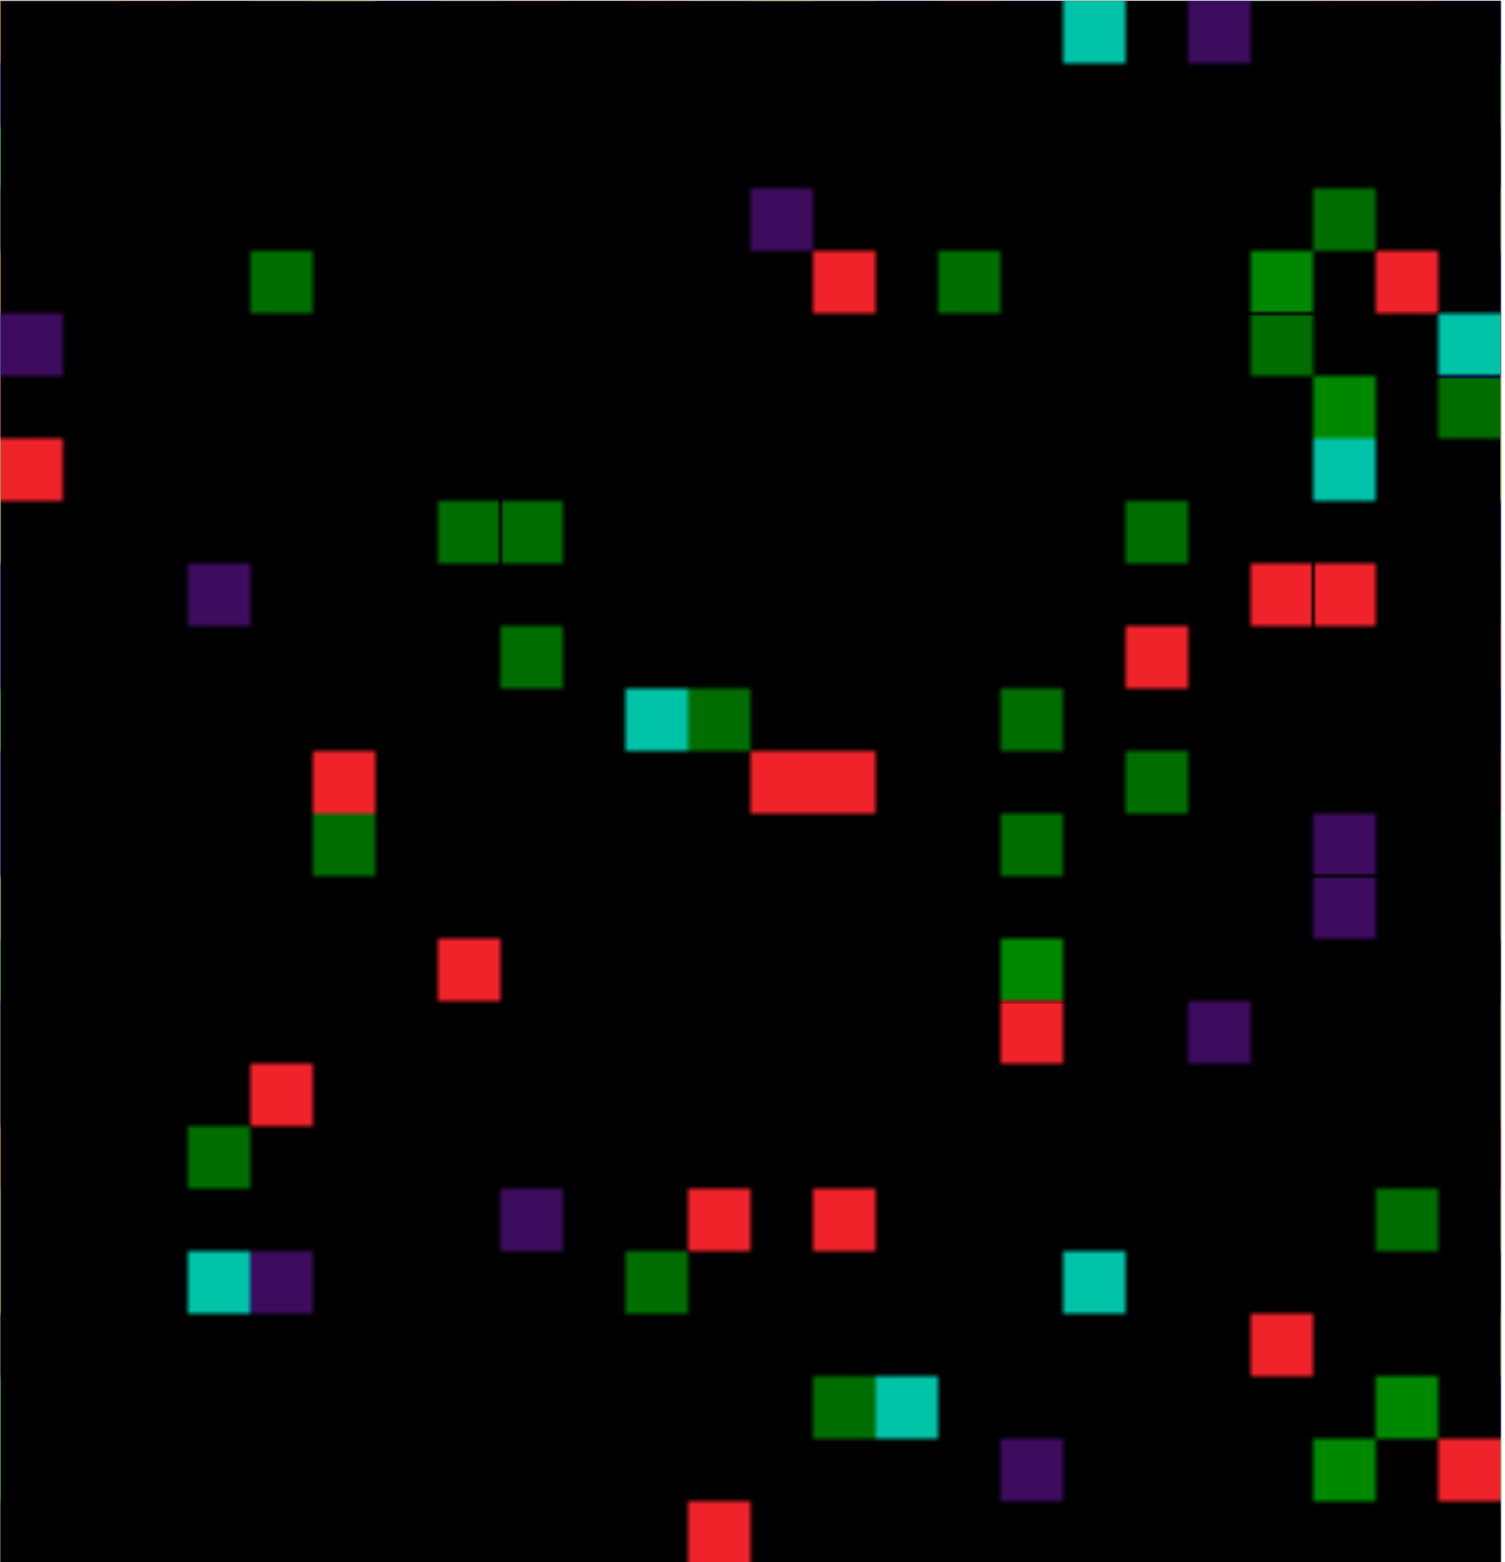
\includegraphics[width=0.2\textwidth]{figs/typical_diff.png}
    \caption{Left: Actual Colors. Center: Colors perceived by typical eyes. Right: Difference between the images}
\end{figure}

\subsubsection{Comparison of Eyes with Varying Levels of Cell Death}

As expected, the image gets noisier as the level of cell death increases, showcasing the decreasing prediction accuracy. Observe that the noise generally consists of colors that are nearby the true color, showing that the eye is still picking up on the trend, but is missing the full acuity needed to perceive the correct color. As the cell death gets near 70\%, however, the original information is lost almost entirely and is taken over by noise.

\begin{figure}[H]
    \centering
    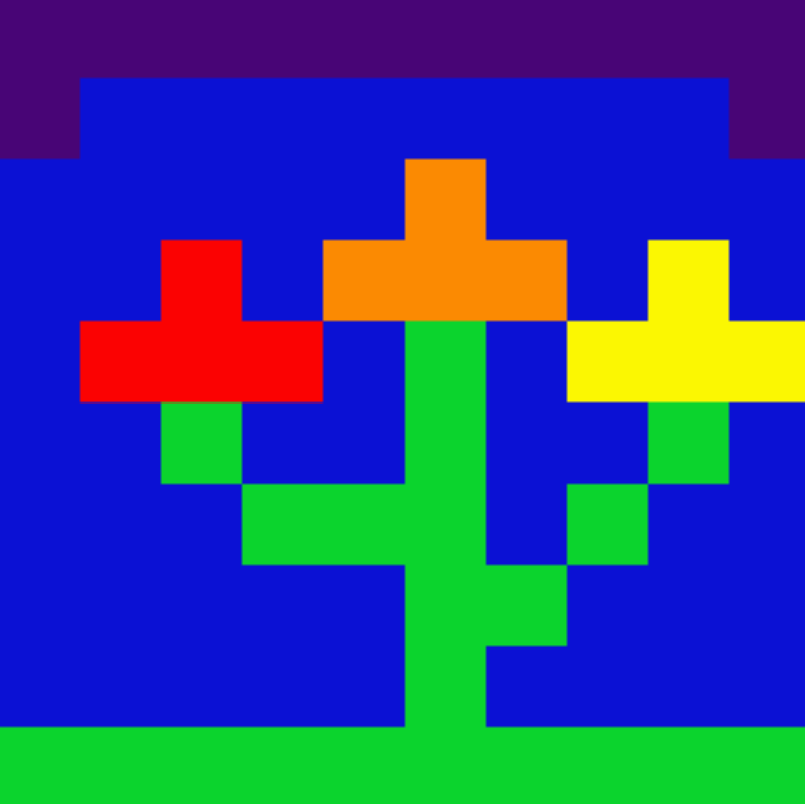
\includegraphics[width=0.2\textwidth]{figs/original_flower.png}
    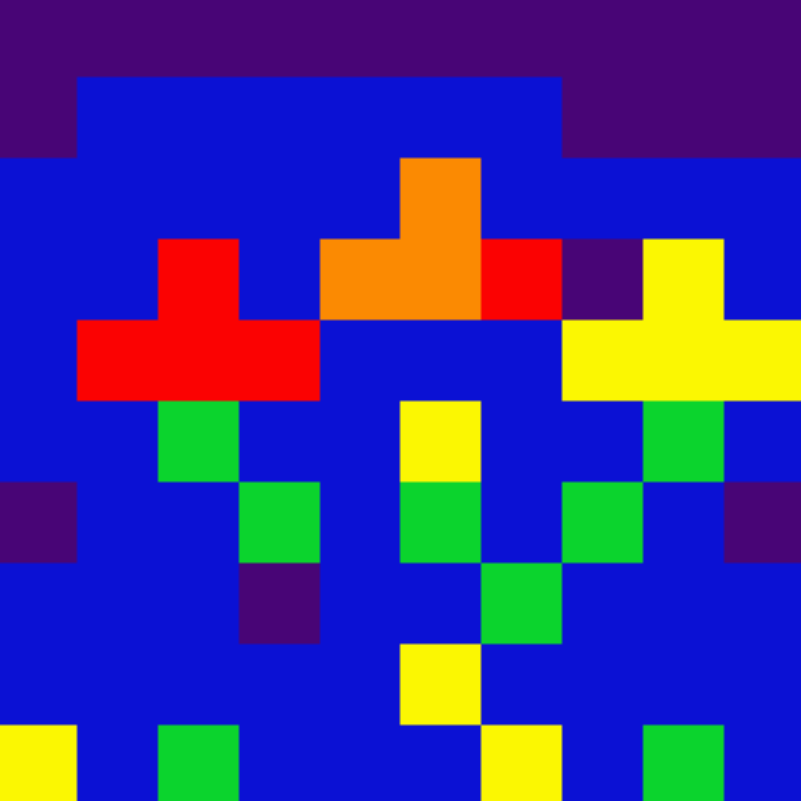
\includegraphics[width=0.2\textwidth]{figs/flower_25.png}
    
\includegraphics[width=0.2\textwidth]{figs/flower_50.png}
    
\includegraphics[width=0.2\textwidth]{figs/flower_75.png}
    \caption{Left to right: Original flower, flower perceived with 25\%, 50\%, and 75\% cell death}
\end{figure}

\begin{figure}[H]
    \centering
    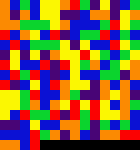
\includegraphics[width=0.2\textwidth]{figs/damage70_actual_results.png}
    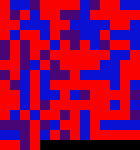
\includegraphics[width=0.2\textwidth]{figs/damage70_predicted_results.png}
    \caption{Left: Actual Colors. Right: Colors perceived by eyes with 70\% cell death}
\end{figure}

\subsubsection{Dichromatic Eyes (2 Cell Types - Red-Green Colorblind)}

Note the decreased accuracy and increased frequency of certain colors, most notably green. Some red/green color confusion is seen, as expected, but colors that were not expected to change as much, such as blue, also have an increased confusion level.

\begin{figure}[H]
    \centering
    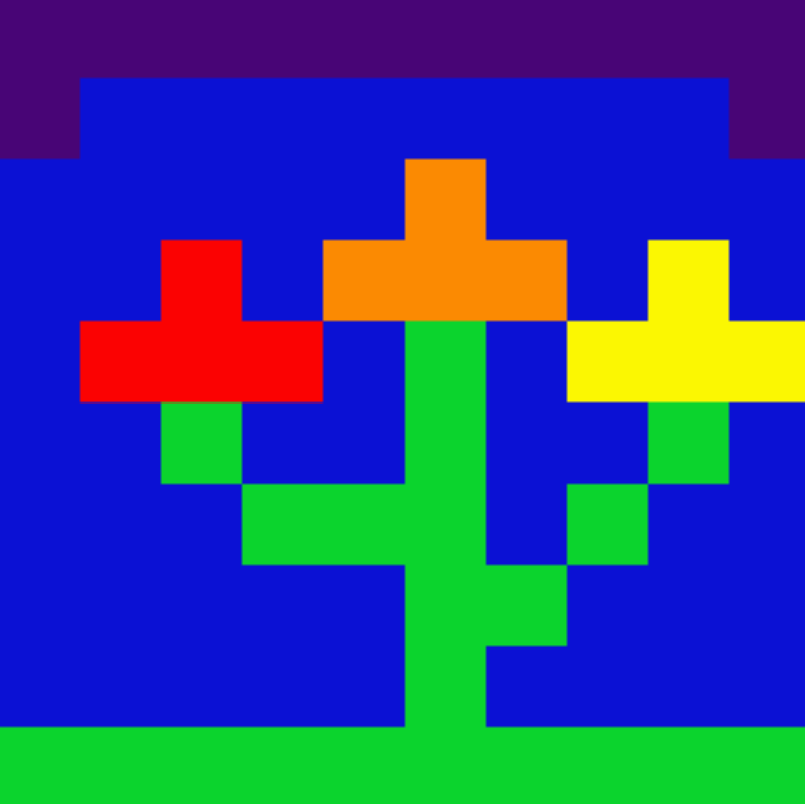
\includegraphics[width=0.2\textwidth]{figs/original_flower.png}
    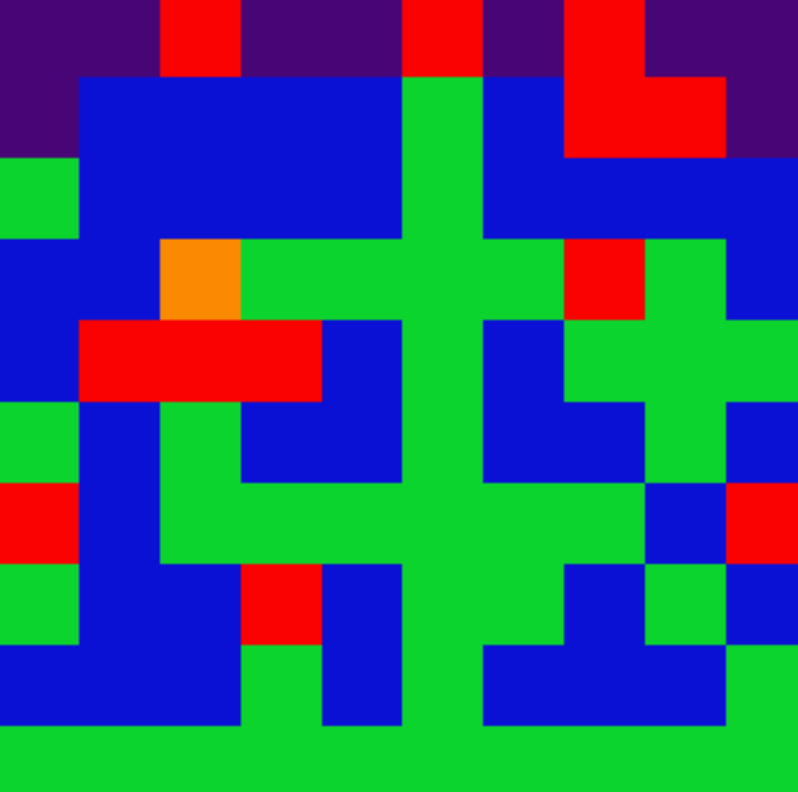
\includegraphics[width=0.2\textwidth]{figs/flower_colorblind.png}
    \caption{Left: Original flower. Right: Flower perceived by colorblind eyes}
\end{figure}

\begin{figure}[H]
    \centering
    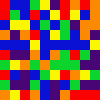
\includegraphics[width=0.2\textwidth]{figs/colorblind_actual_results.png}
    
\includegraphics[width=0.2\textwidth]{figs/colorblind_predicted_results.png}
    \caption{Left: Actual Colors. Right: Colors perceived by colorblind eyes}
\end{figure}

\subsubsection{Tetrachromatic Eyes (4 Cell Types - Additional Color Perception)}

This image comparison showcases how tetrachromacy resulted in a loss of performance where we expected it to be on par or even surpass the trichromatic (typical) eyes. The performance is still much better than the colorblind eye, and general shape is retained.

\begin{figure}[H]
    \centering
    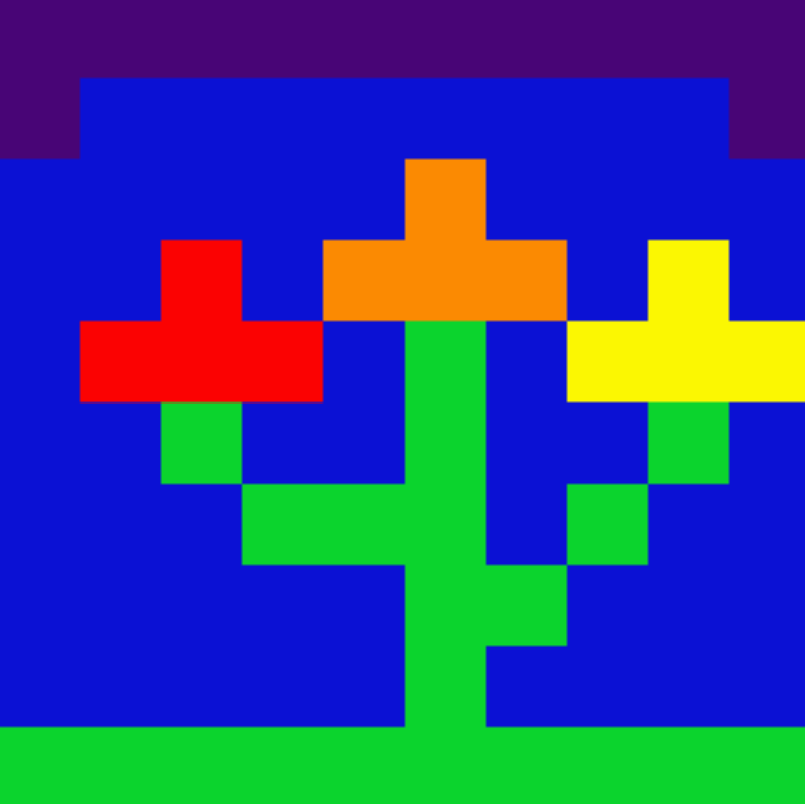
\includegraphics[width=0.2\textwidth]{figs/original_flower.png}
    
\includegraphics[width=0.2\textwidth]{figs/flower_tetra.png}
    \caption{Left: Original flower. Right: Flower perceived by tetrachromatic eyes}
\end{figure}

\begin{figure}[H]
    \centering
    
\includegraphics[width=0.2\textwidth]{figs/tetrachromatic_actual_results.png}
    
\includegraphics[width=0.2\textwidth]{figs/tetrachromatic_predicted_results.png}
    \caption{Left: Actual Colors. Right: Colors perceived by tetrachromatic eyes}
\end{figure}

\section{Discussion}

\subsection{Insights}

Our model's statistical performance met our expectations, but a few parts of it's true behavior were surprising. This was most notable when examining the visualization of model perceptions. 

\bigskip

First, we noted that specific colors were guessed more often than others in cases of uncertainty, and the greatest example of this is the absence of yellow. This is likely due to the difference in wavelength range for the color binning, as yellow has the smallest range. We attempted to combat this, and were partially successful, by selecting a color first from a uniform distribution, then selecting a wavelength from a uniform distribution over that color's range, rather than simply sampling from a uniform distribution over all valid visible wavelengths. 

\bigskip

Another case of unexpected behavior arose when investigating tetrachromatic eyes. In actual human eyes, the additional type of cone cell is believed to provide a richer perception of color and increased acuity in shade differentiation. Our model, however, actually performed worse with tetrachromatic eyes. This may be due to an issue with how we modeled tetrachromacy, or possibly even with the training process for this unique case. 

\bigskip

Also worth noting is that the performance decrease in "colorblind" individuals was expected, but the loss of acuity across the board (resulting in the loss of shape for the visualization) was unexpected. We assumed the behavior would more closely resemble actual colorblindness, where certain colors, particularly red and green, are mistaken, rather than across the board. We could investigate further into why this may be and further improve our modeling of this type of atypical behavior. 

\bigskip

Alternatively, a few cases of expected behavior involves the misidentification of similar colors (mixing up orange/red or blue/purple), the inverse relationship between cell death percentage and accuracy, and the general difference in behavior between eyes with typical and atypical numbers of cone cell types. 

\subsection{Challenges}

\subsubsection{Representation of Cone Cells}

We faced difficulties in how cone cells were represented as input to the model. The path we opted to take was organizing the cone cells by their type (i.e. S, M, or L). This provided good results for typical eyes, but it made colorblind and tetrachromatic eyes more difficult because the cone cell types were no longer the same.

\subsubsection{Tetrachromatic Difficulties}

As mentioned above, we faced difficulties in obtaining the expected performance boost of tetrachromatic eyes, and in fact saw a decrease in performance. This could be explored further, and perhaps tested in conditions that benefit tetrachromacy, such as increasing the number of color classifications, especially for longer wavelengths of light (warmer colors).

\subsection{Future Work}

Additional phenomena could be modeled using this technique by expanding its complexity. One pathway could involve the combined perception of color given multiple wavelengths, or investigating a two-dimensional perception of color by taking both multiple wavelengths and cone cell position into account. This would take in a full "image" at once, and predict a full "image" of color. However, it is very likely that this would greatly increase data dimensionality and model complexity, especially if done in a naive way. 

\bigskip

One example of such phenomena would consist of the inconsistent perception of color given various lighting environments. One classic example of this is "The Dress" sensation from 2015, where, due to a lack of contextual information, different people perceive the dress as being blue and black or white and gold, seen in Figure \ref{fig:the_dress_original} \cite{thedress}. This contextual information has a huge impact on color perception, as the given color of an object at any one time is dependent on \textit{both} it's reflectance properties \textit{and} the lighting conditions. This is showcased in Figure \ref{fig:the_dress}

\begin{figure}[H]
    \centering
    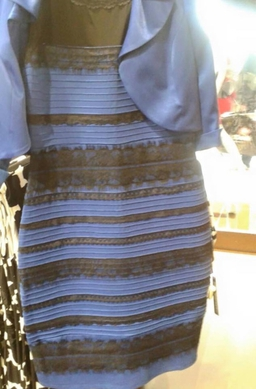
\includegraphics[width=0.25\textwidth]{figs/the_dress_original.jpg}
    \caption{The original photo of the dress \cite{thedress}}
    \label{fig:the_dress_original}
\end{figure}

\begin{figure}[H]
    \centering
    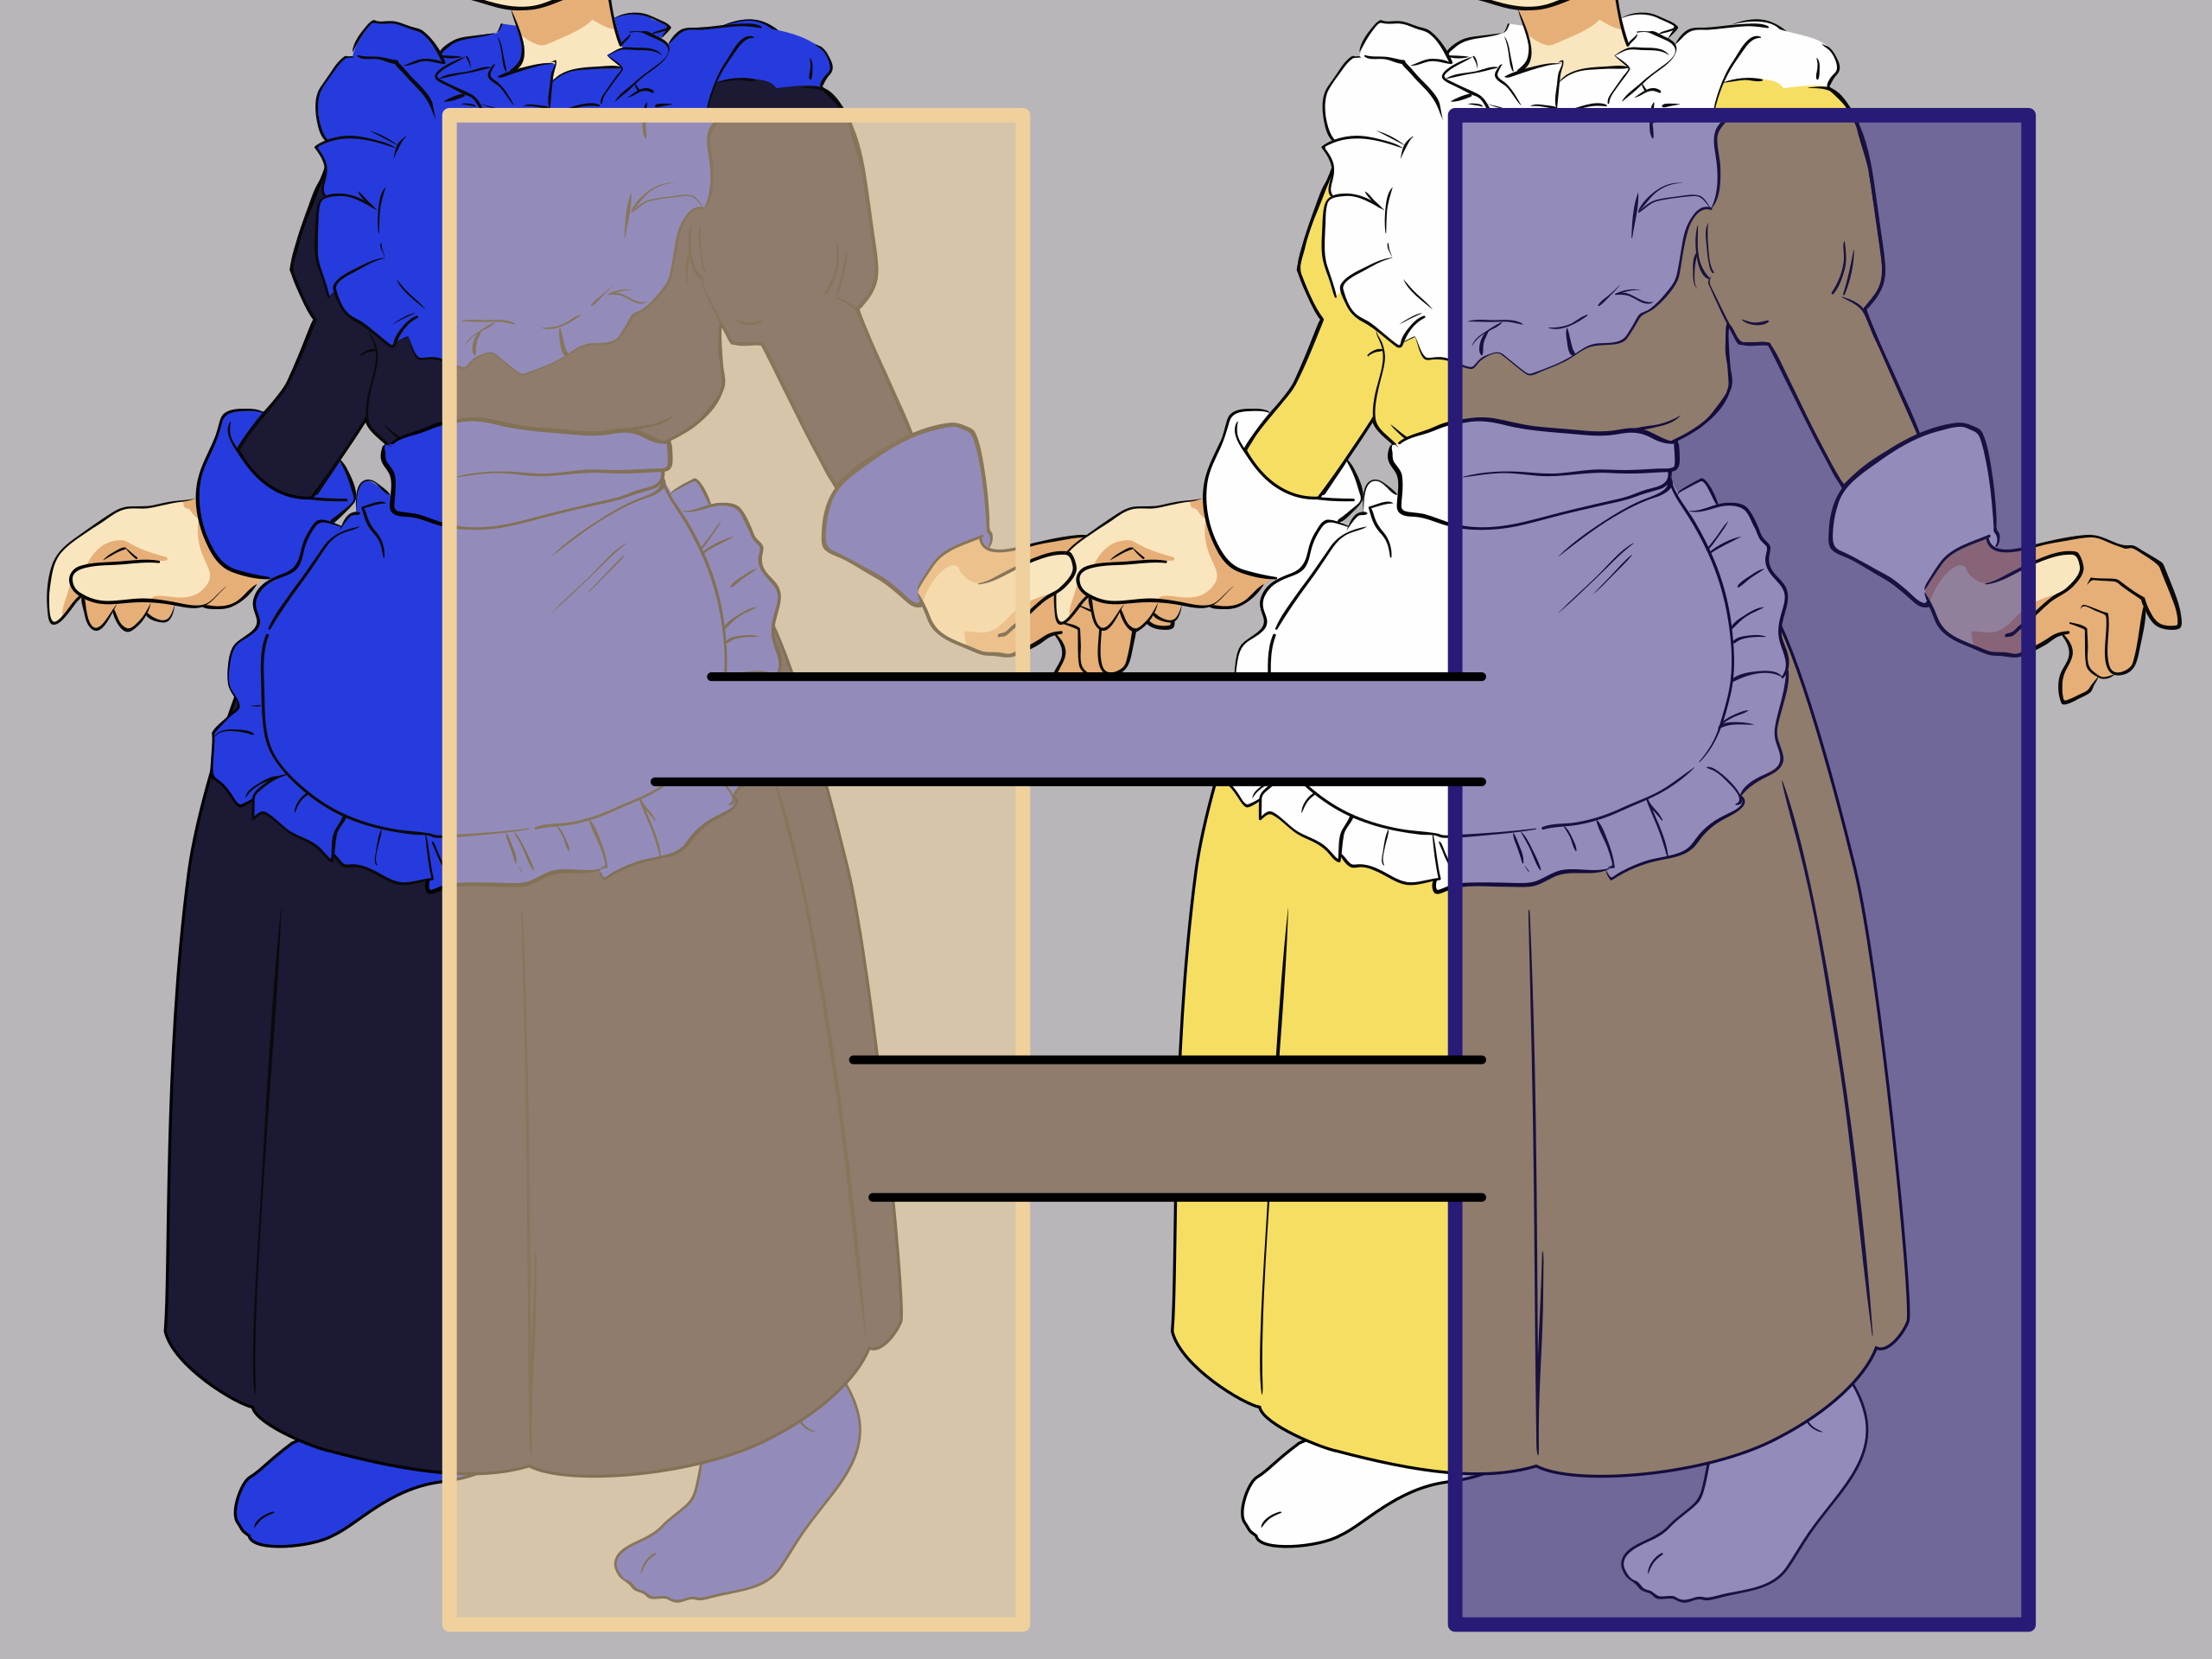
\includegraphics[width=0.45\textwidth]{figs/the_dress.png}
    \caption{Comparison of the perception of the dress given differing lighting conditions \cite{thedress}}
    \label{fig:the_dress}
\end{figure}

Alternatively, other types of atypical eyes could be modeled by looking at how the cone cells for these types of eyes behave. For example, we only looked at an approximation of one kind of colorblindness. Other types of colorblindness and other eye diseases could be modeled. Non-human eyes could also be explored, as other species have different distribution, type, and count of cone cells (and may have more tangible data to compare to).

\bigskip

Of course, improvements to the existing model could be made. The simulation could be refined to better represent cone cells and techniques could be investigated to solve some of the problems we ran into. Additionally, the neural network could also be refined to improve the accuracy of each type of prediction and further eliminate any overfitting.

\section*{Acknowledgments}

We thank Stefan T. Radev for his support in formulating the problem and guidance on the feasibility and process of simulating valid data.

\newpage
\printbibliography[title=References]

\end{document}
